\documentclass[letterpaper]{article}
\usepackage[submission]{aaai2027}

\usepackage[hyphens]{url}
\urlstyle{rm}
\def\UrlFont{\rm}
\usepackage{graphicx}
\usepackage{natbib}
\usepackage{caption}
\usepackage{booktabs}
\usepackage{array}
\usepackage{xspace}
\usepackage{xcolor}
\usepackage{tikz}
\usetikzlibrary{arrows.meta,positioning}
\frenchspacing
\pdfinfo{
/TemplateVersion (2027.1)
}

\newcommand{\sys}{\textsc{AgentProf}\xspace}
\newcommand{\operation}{\texttt{operation}\xspace}
\newcommand{\opstack}{\texttt{operation stack}\xspace}
\providecommand{\Description}[1]{}

\newcommand{\ckupdate}[1]{\textcolor{blue}{#1}}

\begin{document}

\title{AgentProf: Semantic Profiling for AI Agents}
\author{Anonymous Submission}
\affiliations{}

\maketitle

\begin{abstract}
AI agents increasingly orchestrate long-running, multi-step activities involving thousands to millions of interactions with users, tools, and system resources.
% AI 智能体编排涉及数千到数百万次交互的长时间多步骤活动。
To improve quality, safety, and cost efficiency of AI agents, developers need to determine where failures concentrate, which workflows trigger unsafe effects, and which task categories consume the most budget.
% 为提高智能体的质量、安全性和成本效率，开发者需确定故障集中在哪里、哪些工作流触发不安全副作用、哪类任务消耗最多预算。
To answer similar questions in traditional systems software, profiling attributes resource consumption to responsible entities, such as code paths, by aggregation.
% 在传统系统软件中，profiling 通过聚合将资源消耗归因到负责实体（如代码路径）。
Yet existing agent observability tools focus on single-execution debugging and tracing rather than profiling, making these questions difficult to answer as trajectories grow long and complex.
% 然而现有智能体可观测性工具聚焦于单次执行的调试和 tracing 而非 profiling，使这些问题在轨迹变长变复杂时难以回答。
Agent behavior differs from code execution, creating two challenges for profiling: the responsible entities are semantic categories such as task intent and workflow phase, not code paths, and agent trajectories lack the stable identifiers and structural hierarchies that make attribution possible.
% 智能体行为与代码执行不同，给 profiling 带来两个挑战：负责实体是语义类别（如任务意图和工作流阶段）而非代码路径，且智能体轨迹缺乏使归因成为可能的稳定标识符和结构层次。
We propose a \emph{semantic operation stack model} that adapts profiling to agent trajectories.
% 我们提出一个将 profiling 适配到智能体轨迹的语义 operation stack 模型。
Uniform \emph{operations} represent all agent activities, and \emph{operation stacks} replace the runtime call stack, enabling hierarchical attribution at different levels of granularity from the same data.
% 统一的 operation 表示所有智能体活动，operation stack 替代运行时调用栈，使同一数据支持不同粒度的分层归因。
We observe that an agent's task occupies a contiguous span of a trajectory and decomposes into contiguous subtasks, so task structure is a set of nested named intervals recoverable by finding only the transitions between them, and we design \emph{recursive operation segmentation}: it splits a trajectory where the agent's responsibility changes, names the intervals on both sides, and recurses to supply the missing stack.
% 我们观察到智能体的任务占据轨迹上一段连续区间并可分解为连续子任务，因此任务结构是一组嵌套命名区间，只需找出转移点即可恢复；据此我们设计递归 operation 切分：在责任变化处切开轨迹，为两侧区间命名并递归，提供缺失的栈。
\sys implements this in a profiler that compiles local agent trajectories into pprof-compatible profiles.
% \sys 将其实现为一个 profiler，把本地智能体轨迹编译为 pprof 兼容的 profile。
On real trajectories and public datasets, our evaluation shows that semantic profiling effectively attributes cost and locates problems across agent trajectories.
% 在真实轨迹和公开数据集上，评估表明语义 profiling 能有效地跨轨迹归因开销和定位问题。
\end{abstract}

% AI agents increasingly orchestrate long-running, multi-step
% activities involving thousands to millions of interactions with
% users, tools, and system resources.
% To optimize the quality, safety, and cost of agents, developers must 
% analyze behaviors across thousands of runs to 
% find where failures concentrate, 
% locate the workflow phases triggering unsafe effects, 
% and identify the tasks that consumes most budget. 

% While performance profiling traditionally answers these questions 
% for classic software by aggregating resource consumption, 
% traditional profilers fail for agents.
% unlike traditional software where code paths provide a natural hierarchy for profiling, 
% agent behaviors are driven by unstructured natural language prompts 
% and lack deterministic execution stacks. 
% To bridge this gap, we propose the Semantic Operation Stack model. 
% First, we unify all heterogeneous agent activities (prompts, tool calls, 
% and system I/O) into a single structured record called an operation. 
% Second, we construct dynamic call stacks at query time by projecting 
% these operations onto user-defined semantic fields (e.g., intent $\rightarrow$ phase $\rightarrow$ action), merging identical sequences to generate flame graphs.

% We implement this model in AgentProf, an offline profiler 
% with pluggable algorithms for intent attribution and stack construction, 
% compiling local agent trajectories into standard, pprof-compatible profiles.

%% ===================================================================
\section{Introduction}
\label{sec:intro}

\begin{figure}[!t]
\centering
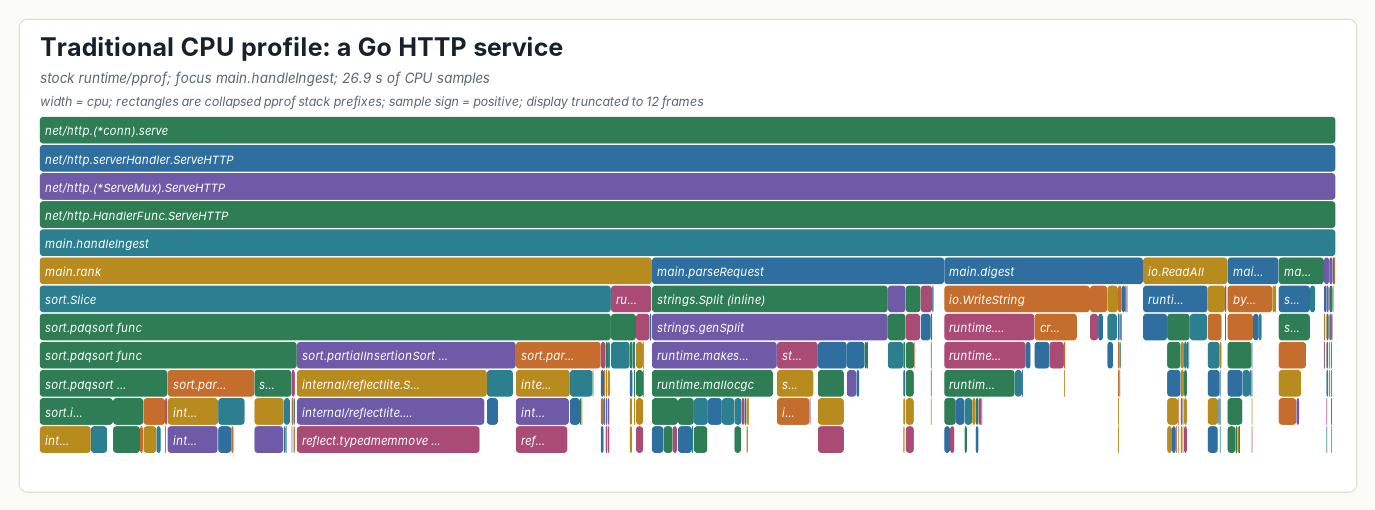
\includegraphics[width=\columnwidth]{figures/go-http-cpu.png}\\[1pt]
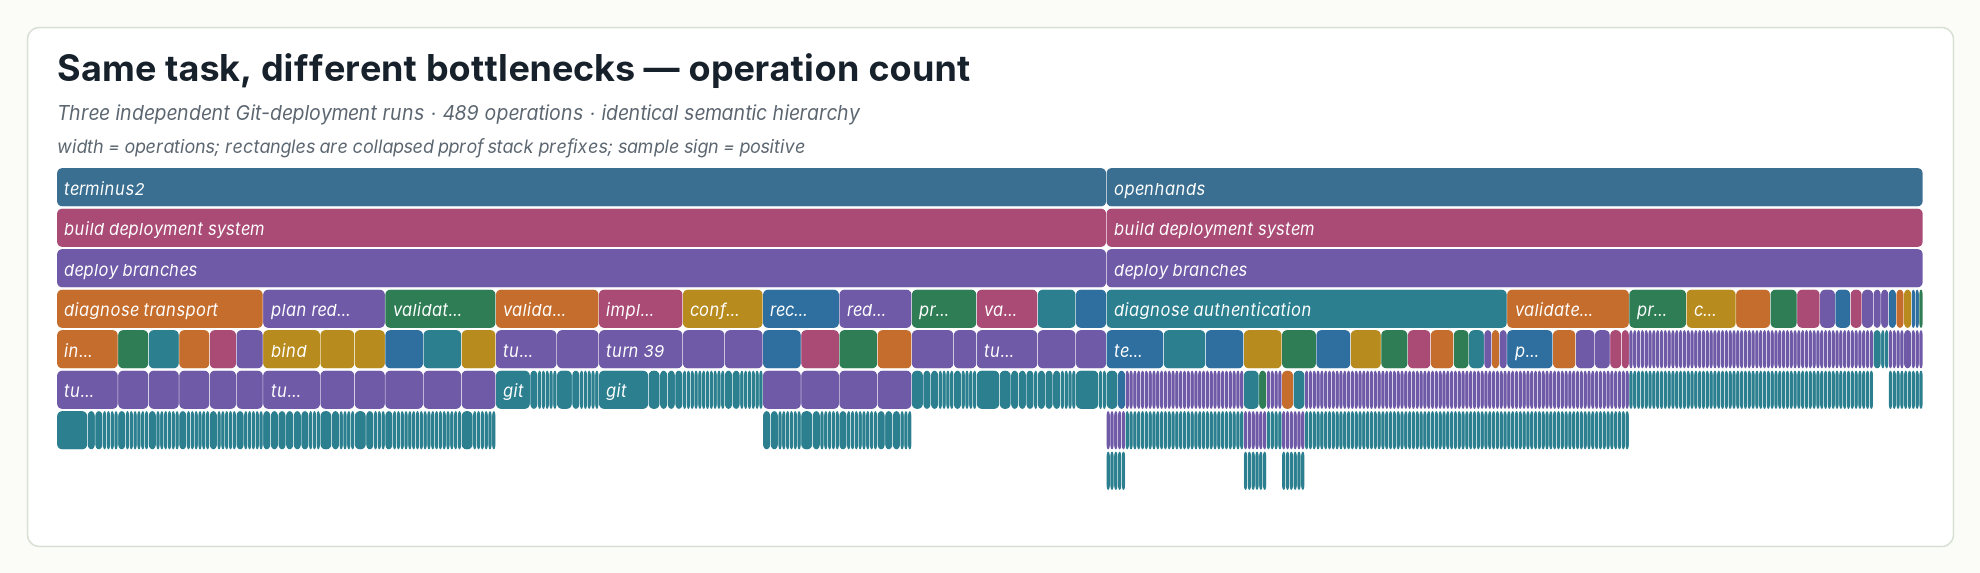
\includegraphics[width=\columnwidth]{figures/git-multibranch.operations.png}\\[1pt]
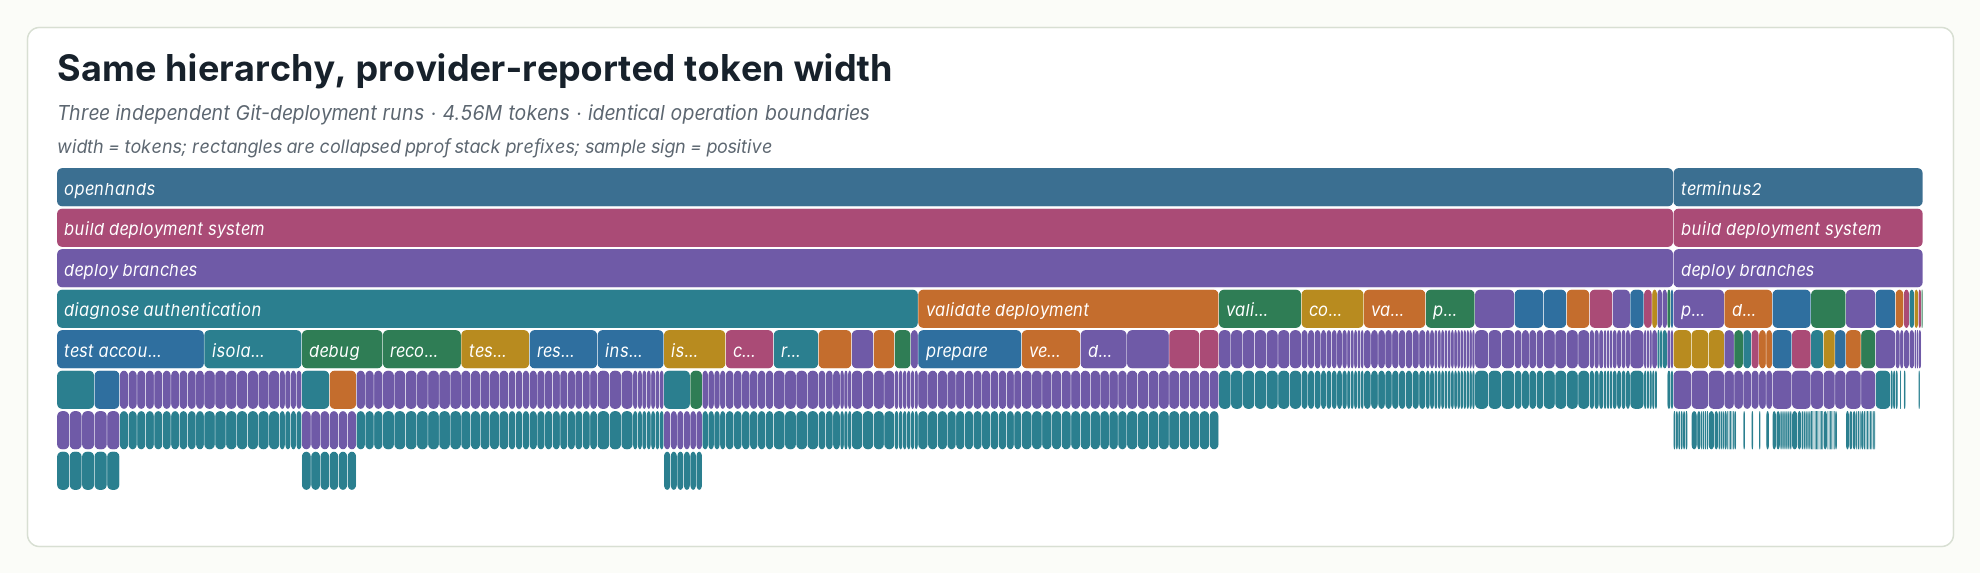
\includegraphics[width=\columnwidth]{figures/git-multibranch.tokens.png}\\[1pt]
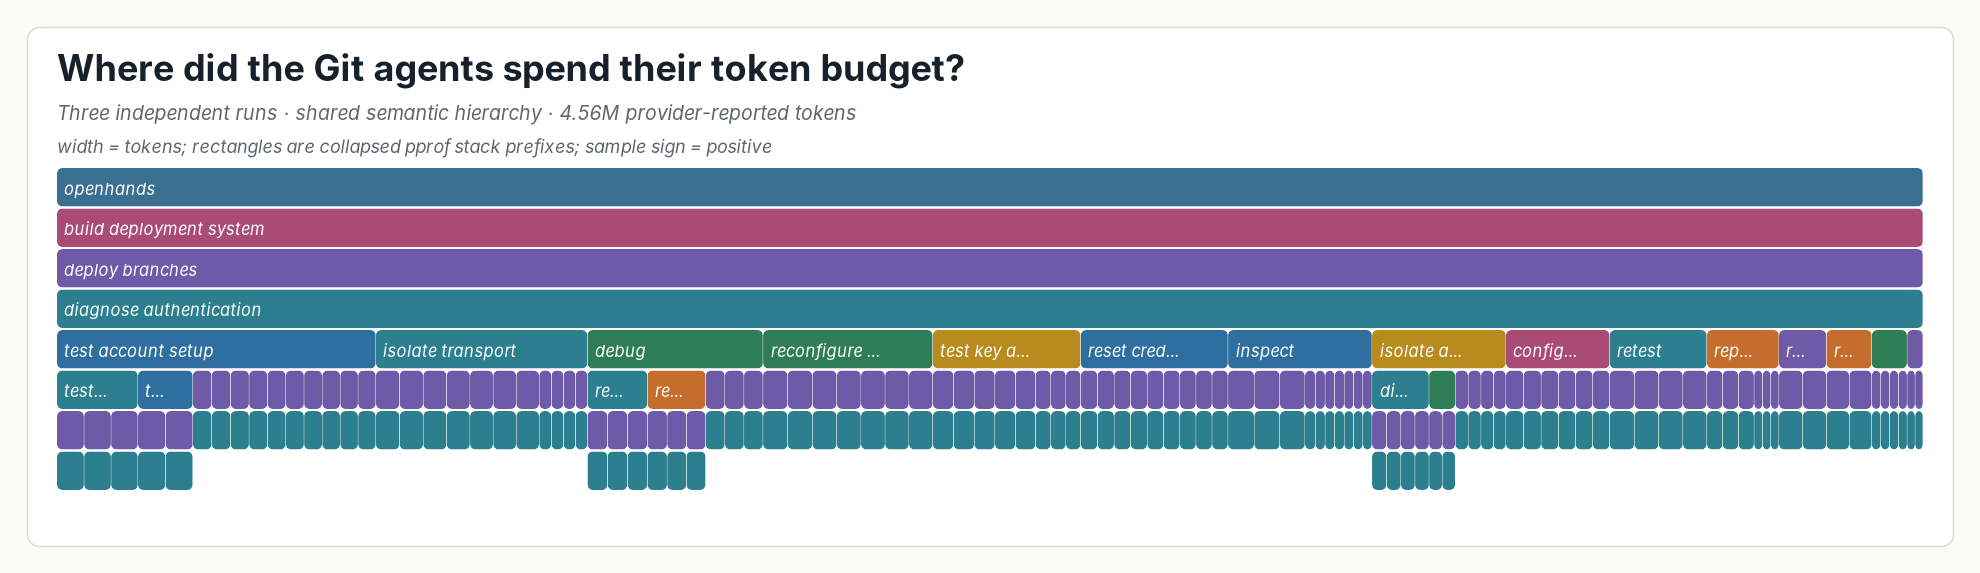
\includegraphics[width=\columnwidth]{figures/git-authentication.tokens.png}
\caption{One renderer, four standard pprof profiles.
\emph{(a)} CPU time in a Go HTTP service.
\emph{(b, c)} Three agent executions of one Git-deployment task under one
fixed operation hierarchy: width is operation count in (b) and tokens in (c).
The hierarchy is identical in both; only the measure changes.
\emph{(d)} The same token profile focused on the shared \texttt{diagnose
authentication} responsibility.
Every panel is read the same way: width is aggregate cost, a parent contains
its children, and identical stacks fold.}
\Description{Four flame graphs in one visual style. The first descends from a
Go HTTP server's connection handler into request handling, ranking, parsing,
and hashing. The second and third show the same agent hierarchy weighted by
operation count and by tokens, where the count view is dominated by one agent
framework and the token view by another together with repeated
authentication diagnosis. The fourth expands that authentication
responsibility into account, transport, credential, and retest operations.}
\label{fig:flamegraph}
\end{figure}

%% ¶1: Background + context
AI agents~\cite{sweagent,claudecode,osworld} orchestrate multi-step activities that span two layers, high-level intent (prompts, LLM calls, tool invocations) and low-level system effects (process spawns, file and network I/O).
% AI 智能体~\cite{sweagent,claudecode,osworld}编排跨越两层的多步骤活动：高层意图（提示词、LLM 调用、工具调用）和低层系统副作用（进程创建、文件和网络 I/O）。
As agents evolve from short, scripted workflows into complex systems that run for hours and days, with a large number of interactions each, production teams accumulate many such trajectories over weeks or months.
% 随着智能体从短小的脚本化工作流进化为每次运行数小时、包含数千次交互的复杂系统，生产团队在数周或数月内积累大量此类轨迹。

%% ¶2: Problem
To improve agent quality, safety, and cost efficiency, developers
need to analyze operational behavior across trajectories and
interactions.
Which categories of tasks consume the most token budget? Where do
failures concentrate across workflows? Which behavioral patterns
trigger unsafe system effects?
% 为了提高智能体质量、安全性和成本效率，开发者需要跨轨迹和交互分析运维行为。哪类任务消耗最多 token 预算？故障跨工作流集中在哪里？哪些行为模式触发不安全系统副作用？
Answering these questions requires analysis and evaluation across many
trajectories~\cite{agentatlas,agentrewardbench}, a task becoming costly for manual inspection or
per-trajectory LLM evaluation~\cite{llm-as-judge} at scale.
% 回答这些问题需要跨许多轨迹的分析和评估，在规模化时人工检查或逐轨迹 LLM 评估的成本越来越高。
In traditional systems software, profiling answers these questions by
attributing resource consumption to responsible entities by
aggregation, as distinct from single-execution debugging and tracing.
% 在传统系统软件中，profiling 通过聚合将资源消耗归因到负责实体来回答这些问题，区别于单次执行调试和 tracing。

%% ¶3: Existing solutions
Yet existing agent tools support debugging and tracing but not
profiling.
% 然而现有智能体工具支持调试和 tracing，但不支持 profiling（Background）。
Some~\cite{langsmith,langfuse,phoenix,otel} organize events into
per-execution span trees, effective for diagnosing a single run but
unable to aggregate by semantic category.
% 一些工具~\cite{langsmith,langfuse,phoenix,otel}将事件组织为按执行划分的 span 树，有效诊断单次运行但无法按语义类别聚合。
Others~\cite{datadog-llmobs,laminar-signals} cluster inputs or
extract structured signals, but characterize \emph{input
distributions} (``30\% of users ask code questions'') rather than
\emph{resource attribution} (``review tasks consume 40\% of the
token budget''), because tags at the request level do not propagate
to downstream tool calls and system effects.
% 另一些~\cite{datadog-llmobs,laminar-signals}聚类输入或提取结构化信号，但刻画的是输入分布（"30\% 的用户提问代码问题"）而非资源归因（"review 任务消耗了 40\% 的 token 预算"），因为请求级的标签不会传播到下游工具调用和系统副作用。

%% ¶4: Challenge — why traditional profiling doesn't transfer directly
Adapting profiling to agent trajectories is challenging.
% 将 profiling 适配到智能体轨迹具有挑战性（Background）。
In traditional software, the responsible entities are code paths.
Profiling is straightforward because function names are
stable and runtime call nesting provides the attribution
hierarchy.
% 在传统软件中，负责实体是代码路径。Profiling 是直接的，因为函数名是稳定的，运行时调用嵌套提供归因层次。
Agent behavior differs fundamentally.
To answer the questions above, the responsible entities need to be
semantic categories such as task intent and tool operation, not code
paths.
% 智能体行为有根本不同。要回答上述问题，负责实体需要是语义类别（如任务意图和工具操作），而非代码路径。
Agent trajectories lack the two properties that make traditional profiling possible.
% 智能体轨迹缺乏使传统 profiling 成为可能的两个特性。
Prompts are natural language, so two prompts expressing the same intent share no common string.
% 提示词是自然语言，表达相同意图的两个提示词没有共同字符串。
Agent events have no runtime call-stack hierarchy because prompts,
tool calls, and system effects are not nested by execution the way
function calls produce stack frames: a sequence of prompts can be a task or multiple tasks, a task can be part of a bigger task.
% 智能体事件没有运行时调用栈层次，因为提示词、工具调用和系统副作用不像函数调用那样通过执行嵌套产生栈帧。

%% ¶5: Model
Despite these differences, the fundamental profiling methodology
transfers to agent trajectories: project resources onto responsible
entities, assign stable tags, and attribute hierarchically.
% 尽管有这些差异，基本的 profiling 方法论可以迁移到智能体轨迹：将资源投影到负责实体、赋予稳定标签、分层归因。
We propose a \emph{semantic operation stack model} with two
components.
% 我们提出一个包含两个组件的语义 operation stack 模型。
\emph{Operations} are uniform records with string fields and
additive measures that represent all agent activities (prompts, LLM
calls, tool invocations, and system effects) without type-specific
objects.
% Operation 是带有字符串字段和可加度量的统一记录，表示所有智能体活动（提示词、LLM 调用、工具调用和系统副作用），无需特定类型对象。
\emph{Operation stacks} provide hierarchical attribution, replacing the runtime call stack.
% Operation stack 提供分层归因，替代运行时调用栈。
Choosing different fields changes the attribution granularity: the same operations can be attributed by task category, by execution phase, by session, or by action type, and one fixed hierarchy replays under any additive measure (Figure~\ref{fig:flamegraph}).
% 选择不同字段改变归因粒度：同一组 operation 可按任务类别、执行阶段、会话或操作类型归因，且同一个固定层次可在任意可加度量下重放（Figure~\ref{fig:flamegraph}）。

%% ¶6: This paper + system + results
We implement this model in \sys, an offline profiler that compiles
local agent trajectories into pprof-compatible profiles
(Figure~\ref{fig:architecture}).
% 我们在 \sys 中实现此模型，这是一个离线 profiler，将本地智能体轨迹编译为 pprof 兼容的 profile（Figure~\ref{fig:architecture}）。
One algorithm supplies the tags the trajectory does not carry, and its
design follows from one observation about agent work: a task occupies a
contiguous span of a trajectory and decomposes into contiguous subtasks,
so task structure is exactly a set of nested named intervals, and
recovering it requires only finding the transitions between them.
% 一个算法提供轨迹本身没有的标签，其设计源于一个关于智能体工作的观察：任务占据轨迹上一段连续区间并分解为连续的子任务，因此任务结构恰好是一组嵌套的命名区间，恢复它只需找到它们之间的转移点。
This makes the problem segmentation rather than classification: no
predefined taxonomy is required, and each branch's depth emerges from
the content instead of a fixed schema.
% 这使问题成为切分而非分类：不需要预定义的分类体系，每个分支的深度由内容决定而非由固定 schema 规定。
\emph{Recursive operation segmentation} therefore reads a trajectory,
cuts it at the points where the agent's responsibility changes, names
the intervals on both sides, and recurses, so short verb-led names (like \texttt{diagnose authentication})
give agents the stable identifiers that traditional profiling gets for
free from function names.
% 一个算法驱动此模型：递归 operation 切分通读轨迹，在智能体责任变化处切开，为两侧区间命名并递归；动词优先的短名称为智能体提供了传统 profiling 从函数名免费获得的稳定标识符。
The segmentation interface is implementation-neutral: an agent, a language model, or a statistical rule can all produce the same marks.
% 切分接口与实现无关：agent、普通语言模型或统计规则都能产出相同的标记。
Across all 405 released CodeTraceBench~\cite{li2026codetracer} trajectories, recursive
segmentation agrees with human stage annotations at 0.764
B$^3$ F1~\cite{bagga-baldwin-1998-entity-based}, versus 0.663 for a statistical baseline and 0.541 for raw
actions.
% 在全部 405 条已发布的 CodeTraceBench 轨迹上，递归切分与人工 stage 标注的普通 B$^3$ F1 一致性为 0.764，统计基线为 0.663，raw action 为 0.541。
On three complete localization benchmarks, the profile improves ranking over each benchmark's own diagnostic, raising MAP by 0.031, 0.107, and 0.117.
% 在三个完整定位 benchmark 上，profile 改进了排序，相对各 benchmark 自带诊断将 MAP 分别提高 0.031、0.107 与 0.117。
As a navigation aid, it helps a reader reach equal ranking quality while opening 53.0\% instead of 65.0\% of the source evidence.
% 作为导航辅助，它帮助读者在只打开 53.0\%（对 65.0\%）source evidence 的情况下达到同等排序质量。
One fixed hierarchy replays under operation-count and token measures
with exact conservation, exposing bottlenecks that a count view
understates by more than a factor of two.
% 同一固定层次在 operation 数与 token 两种度量下精确守恒地重放，暴露出 count 视图低估两倍以上的瓶颈。

%% ¶7: Contributions
This paper makes three contributions:
% 本文做出三项贡献：

\begin{enumerate}
\item \textbf{Semantic operation stack model.}
  We identify the missing profiling layer in agent observability and
  propose a model of uniform operations and query-time operation
  stacks (Background and Design).
% 语义 operation stack 模型。识别智能体可观测性中缺失的 profiling 层，提出统一 operation 和查询时 operation stack 的模型。
\item \textbf{System: \sys.}
  A profiler that implements this model, producing pprof-compatible output.
% 系统：\sys。实现此模型的 profiler，产生 pprof 兼容输出。
\item \textbf{Evaluation.}
  We evaluate profiler output against independent ground-truth
  annotations that stay hidden from the profiler, on eight public
  benchmarks and three real trajectory populations.
% 评估。将 profiler 输出与对 profiler 隐藏的独立真实标注评分，在八个公开 benchmark 与三个真实轨迹 population 上验证。
\end{enumerate}

%% ===================================================================
\section{Background and Motivation}
\label{sec:background}

\subsection{LLMs and AI Agents}
% AI 智能体

A typical agent trajectory interleaves two layers of activity.
% 典型的智能体轨迹交织两层活动。
At the intent layer, the agent receives a user prompt, issues LLM
calls, and invokes tools (code execution, web search, file editing).
% 在意图层，智能体接收用户提示词、发出 LLM 调用并调用工具（代码执行、网络搜索、文件编辑）。
Each tool invocation triggers system effects at the lower layer:
process spawns, file reads and writes, and network requests.
% 每次工具调用在下层触发系统副作用：进程创建、文件读写和网络请求。
A single trajectory may contain hundreds of such intent-effect
cycles, and a production team accumulates many trajectories over
time.
% 单条轨迹可能包含数百个这样的意图-副作用循环，生产团队随时间积累许多轨迹。

\subsection{System Profiling}
% 系统 Profiling

Profiling attributes resource consumption to responsible entities by
aggregation, as distinct from single-execution debugging and
tracing.
% Profiling 通过聚合将资源消耗归因到负责实体，区别于单次执行调试和 tracing。
In traditional software, the profiling pipeline works as follows:
a profiler periodically samples execution state, attaches each
sample to the current call stack, and merges samples with identical
stacks.
% 在传统软件中，profiling 管线如下工作：profiler 周期性采样执行状态，将每个样本附加到当前调用栈，合并具有相同栈的样本。
Flame graphs~\cite{flamegraphs} and pprof~\cite{pprof} call graphs
visualize the result, where width or node size represents aggregate
cost.
% 火焰图~\cite{flamegraphs}和 pprof~\cite{pprof} 调用图可视化其结果，宽度或节点大小代表聚合开销。
Perfetto~\cite{perfetto} generalizes this with SQL-based analysis
and derived events.
% Perfetto~\cite{perfetto} 通过基于 SQL 的分析和衍生事件进行泛化。
These tools support flexible aggregation, but they all assume
stable function names and a runtime call stack.
% 这些工具支持灵活聚合，但都假设稳定的函数名和运行时调用栈。
Pprof's \texttt{tagroot}/\texttt{tagleaf} options can add
label-derived pseudo-frames, but only on top of an existing execution
stack that agent trajectories do not have.
% Pprof 的 \texttt{tagroot}/\texttt{tagleaf} 选项可以添加标签衍生的伪帧，但仅在智能体轨迹不具备的已有执行栈之上。

\subsection{A Motivating Case}
% 动机案例

Three independent agent attempts at one real Git-deployment task all failed to deliver the requested password-authenticated endpoint.
% 同一个真实 Git 部署任务的三次独立 agent 尝试都未能交付所要求的密码认证端点。
The developer's question: \emph{what went wrong, and is it the same problem across all three runs?}
% 开发者的问题：出了什么问题？三次执行是同一个问题吗？
Reading three transcripts totaling 489 operations and 4.6M tokens would take hours.
% 阅读共 489 个 operation、460 万 token 的三份转录需要数小时。
Figure~\ref{fig:flamegraph} places a conventional CPU profile beside the
semantic profile of those three runs.
% 图~\ref{fig:flamegraph} 把一个传统 CPU profile 与这三次执行的语义 profile 并置。
Both are standard pprof profiles drawn by one renderer and read by identical
rules: width is aggregate cost, a parent contains its children, and identical
stacks recorded at different moments fold into one frame.
% 两者都是标准 pprof profile、由同一个渲染器绘制、按完全相同的规则阅读：宽度是聚合开销，父 frame 包含其子 frame，不同时刻记录的相同栈折叠为同一个 frame。
What differs is where the frames come from.
% 差别在于 frame 从哪里来。
A call stack supplies \texttt{net/http.(*conn).serve} at every sample for
free; nothing in an agent trajectory supplies \texttt{diagnose
authentication}, because the three runs express that intent through different
prompts and different shell commands.
% 调用栈在每个样本上免费提供 \texttt{net/http.(*conn).serve}；而智能体轨迹不会提供 \texttt{diagnose authentication}，因为三次执行用不同的提示词和不同的 shell 命令表达同一意图。
Once that name is constructed, the profile answers the engineer's question
directly.
% 一旦这个名字被构造出来，profile 就直接回答了工程师的问题。

The profile answers in one view (Figure~\ref{fig:flamegraph}): all three runs share a \texttt{diagnose authentication} responsibility that consumes 46\% of their combined token budget but only 21\% of operation count.
% profile 用一个视图回答（Figure~\ref{fig:flamegraph}）：三次执行共享一个 \texttt{diagnose authentication} 责任，消耗 46\% 的 token 预算但只占 21\% 的 operation 数。
Drilldown shows all three executions verifying substitute transport paths without ever establishing the target endpoint.
% 下钻显示三次执行都在验证替代传输路径，却从未建立目标端点。
The insight: the agents kept retrying SSH variants instead of fixing the actual credential issue, and operation count alone would hide this because authentication commands are cheap to issue but expensive to verify.
% 洞察：agent 不断重试 SSH 变体而非修复实际凭证问题；仅看 operation 数会掩盖这一点，因为认证命令发起成本低但验证成本高。

A control experiment replays the same operations under native call trees and coarse action grouping: the authentication work scatters across 105 native calls and six action kinds (102 of 105 labeled merely \texttt{run}), but only semantic organization reunites it into one focusable cross-run path.
% 对照实验在 native call tree 和 coarse action 分组下重放相同 operation：认证工作散落于 105 个 native call 和六个 action kind（其中 102 个仅标为 \texttt{run}），只有语义组织将其重聚为一条可聚焦的跨运行路径。
This paper's evaluation returns to this case under RQ1 and asks whether the same behavior holds at population scale.
% 本文的评估在 RQ1 中回到该案例，并检验同样的行为是否在 population 尺度上成立。

\subsection{Challenges for Agent Profiling}
% 智能体 Profiling 的挑战

Existing tools~\cite{langsmith,langfuse,phoenix,otel} record agent
events as per-execution span trees, effective for debugging a single
run.
% 现有工具~\cite{langsmith,langfuse,phoenix,otel}将智能体事件记录为按执行划分的 span 树，有效调试单次运行。
AgentSight~\cite{agentsight} bridges intent and system-effect layers
by correlating eBPF-captured system events with intercepted LLM
traffic, but the resulting recordings still lack aggregate profiling.
% AgentSight~\cite{agentsight} 通过关联 eBPF 捕获的系统事件与拦截的 LLM 流量来桥接意图层和系统副作用层，但生成的记录仍缺乏聚合分析能力。


Adapting profiling to agent trajectories faces two core challenges.
% 将 profiling 适配到智能体轨迹面临两个核心挑战。
The first is that the responsible entities differ.
% 第一个挑战是负责实体不同。
In traditional software, profiling attributes cost to code paths, but
in agent trajectories the relevant entities are semantic categories
such as task intent and workflow phase.
% 在传统软件中，profiling 将开销归因到代码路径，但在智能体轨迹中，相关实体是语义类别（如任务意图和工作流阶段）。
Existing tools~\cite{otel,openinference} do not capture these categories because prompts are natural language: two prompts and tool invocations expressing the same intent may be different, so the profiler cannot aggregate them the way it aggregates identical function names.
% 现有工具无法捕获这些类别，因为提示词是自然语言：表达相同意图的两个提示词可能措辞不同，因此分析器无法像聚合相同函数名那样聚合它们。
The second challenge is that agent trajectories have no runtime hierarchy for attribution.
% 第二个挑战是智能体轨迹没有运行时归因层次。
In CPU profiling, the call stack determines attribution at every level: \texttt{malloc}'s cost belongs to \texttt{parse}, to \texttt{process}, and to \texttt{main} simultaneously.
% 在 CPU 分析中，调用栈决定了每个层级的归因：\texttt{malloc} 的开销同时属于 \texttt{parse}、\texttt{process} 和 \texttt{main}。
A sequence of prompts may constitute one task or several, and a task may be part of a larger workflow, but no runtime mechanism marks these boundaries or determines at which granularity to attribute cost.
% 一串提示词可能构成一个任务也可能是多个任务，一个任务可能是更大工作流的一部分，但没有运行时机制标记这些边界或决定在哪个粒度归因开销。
We quantify this in RQ1.
% 我们在 RQ1 (Evaluation) 中量化了这一点。

\subsection{Design Requirements for Agent Profiling}
% 智能体 Profiling 的设计需求

Traditional profiling relies on three mechanisms that the call stack provides automatically.
% 传统 profiling 依赖调用栈自动提供的三种机制。
Agent profiling needs all three but must achieve them without a call stack:
% 智能体 profiling 需要这三种机制，但必须在没有调用栈的情况下实现：

\begin{description}
\item[R1: Cross-layer resource projection.]
In traditional profiling, each sample is taken inside a call context, so resource consumption is automatically attributed to the code path that caused it.
% 在传统 profiling 中，每个采样在调用上下文内完成，因此资源消耗自动归因到造成它的代码路径。
Agent activities span two layers: intent (prompts, LLM calls) and system effects (file I/O, process spawns).
% 智能体活动跨越两层：意图（提示词、LLM 调用）和系统副作用（文件 I/O、进程创建）。
The profiler must connect system-layer resource consumption to intent-level semantic categories.
% 分析器必须将系统层的资源消耗连接到意图层的语义类别。
\item[R2: Stable tags for folding.]
In traditional profiling, function names are stable identifiers that enable folding identical stacks.
% 在传统 profiling 中，函数名是稳定标识符，能够折叠相同的栈。
Agent prompts are natural language, so the profiler must derive short, stable, repeatable tags before folding.
% 智能体提示词是自然语言，因此分析器必须在折叠前派生短小、稳定、可重复的标签。
\item[R3: Hierarchical attribution.]
In traditional profiling, the runtime call stack provides the attribution hierarchy: function calls nest, and folding identical stacks produces the tree that profiles visualize.
% 在传统 profiling 中，运行时调用栈提供归因层次：函数调用嵌套，折叠相同的栈产生 profile 可视化的树。
Agent events are not nested by execution, so the profiler must construct attribution hierarchies from the data.
% 智能体事件没有执行嵌套，因此分析器必须从数据中构造归因层次。
\end{description}

%% ===================================================================
\section{Design}
% 设计
\label{sec:design}

The three requirements (cross-layer resource projection, stable tags, and hierarchical attribution) drive the design.
% 三个需求（跨层资源投影、稳定标签和分层归因）驱动了设计。
Operations satisfy R1 by representing intent and system-effect activities in a single record with tag inheritance, so intent tags propagate to the system effects they trigger.
% Operation（Design）通过将意图和系统副作用活动表示在带标签继承的单一记录中满足 R1，使意图层标签传播到其触发的系统副作用。
\emph{Recursive operation segmentation} satisfies R2 and R3 together: it derives short, stable interval names from trajectory content and nests those intervals into the attribution hierarchy that replaces the runtime call stack.
% 递归 operation 切分（Design）同时满足 R2 与 R3：它从轨迹内容派生短小稳定的区间名称，并将这些区间嵌套为替代运行时调用栈的归因层次。
\emph{Operation stacks} then attribute resources at every level of that hierarchy at query time, so the same data supports multiple views without rebuilding the input.
% Operation stack（Design）随后在查询时沿该层次的每一层归因资源，使同一数据支持多种视图而无需重建输入。
The profiling pipeline has four stages: (1)~parse raw trajectories into operations, (2)~segment trajectories into named nested intervals (or apply mapping rules), (3)~project each operation onto a stack frame sequence chosen at query time, and (4)~fold operations with identical stacks, summing their weights.
% 分析管线有四个阶段：(1) 将原始轨迹解析为 operation，(2) 将轨迹切分为命名嵌套区间（或应用映射规则），(3) 将每个 operation 投影到查询时选择的栈帧序列上，(4) 折叠具有相同栈的 operation 并求和权重。

\subsection{Semantic Operation Stack Model}
% 语义 Operation Stack 模型
\label{sec:ops}

%% ¶1: Operations
Because agent activities span both intent and system-effect
layers, a profiler should not distinguish between them in the
data representation.
% 由于智能体活动跨越 Background 中描述的意图层和系统副作用层，分析器不应在数据表示层面区分它们。
\sys therefore represents every activity as a single abstraction, the
\operation, a weighted record with string fields and additive
measures.
% 因此 \sys 将每个活动表示为单一抽象——operation，一个带有字符串字段和可加度量的加权记录。
Each operation carries string fields (\texttt{project},
\texttt{agent}, \texttt{session}, \texttt{prompt\_tag},
\texttt{kind}, \texttt{model}, \texttt{path}, \texttt{domain},
\texttt{status}, \ldots) and additive measures (token count,
duration, event count).
% 每个 operation 携带字符串字段（\texttt{project}、\texttt{agent}、\texttt{session}、\texttt{prompt\_tag}、\texttt{kind}、\texttt{model}、\texttt{path}、\texttt{domain}、\texttt{status} 等）和可加度量（token 数、持续时间、事件数）。
A prompt, an LLM call, a tool invocation, a file read, a GUI click,
and a process event are all operations with the same schema, distinguished only by which fields carry values.
% 提示词、LLM 调用、工具调用、文件读取、GUI 点击和进程事件都是具有相同 schema 的 operation，仅通过哪些字段有值来区分。

%% ¶2: Operation Stacks
\label{sec:stacks}
An \opstack provides hierarchical attribution for agent trajectories, replacing the runtime call stack.
% 一个 operation stack 为智能体轨迹提供分层归因，替代运行时调用栈。
In CPU profiling, the call stack determines which code paths
share responsibility for a resource cost.
% 在 CPU 分析中，调用栈决定哪些代码路径共同承担资源开销。
An operation stack serves the same role: an ordered list of fields
$[f_1, f_2, \ldots, f_k]$ projects each operation $o$ to a frame
sequence $\langle o.f_1, o.f_2, \ldots, o.f_k \rangle$, and
operations with identical sequences are merged, summing their
weights.
% Operation stack 承担相同角色：有序字段列表 $[f_1, f_2, \ldots, f_k]$ 将每个 operation $o$ 投影到帧序列 $\langle o.f_1, o.f_2, \ldots, o.f_k \rangle$，具有相同序列的 operation 被合并，权重求和。
Unlike a call stack, the fields are chosen at query time, not
determined by execution.
% 与调用栈不同，字段在查询时选择，而非由执行决定。
The same operations can therefore be attributed as a flat task summary, a
per-session tree, a semantic phase/action hierarchy, or a
trajectory using the dataset's own annotations, and changing the fields changes the
attribution without changing the data.
% 因此同一组 operation 可归因为扁平任务摘要、固定会话树、语义阶段/操作层次或使用数据集自身标注的轨迹，改变字段即改变归因方式而无需改变数据。
Sessions and spans are optional operation fields, not fixed hierarchy levels, so the same data supports both debugging views
(include \texttt{session}) and aggregate profiling views (exclude
it).
% 会话和 span 是可选的 operation 字段而非固定层次级别，因此同一数据既支持调试视图（包含 \texttt{session}）也支持聚合 profiling 视图（排除它）。
The frame sequence need not come from fields alone: recursive
segmentation supplies each operation's covering
interval-name chain as a variable-depth frame sequence, and field lists
and interval paths compose in one stack.
% 帧序列不必只来自字段：递归切分（Design）为每个 operation 提供其覆盖区间的名称链，作为可变深度的帧序列；字段列表与区间路径可在同一栈中组合。
A view is a triple $(\varphi, \sigma, w)$: a predicate
$\varphi$ selects which operations participate, a stack function
$\sigma = [f_1, \ldots, f_k]$ maps each operation to its frame
sequence, and a weight function $w$ assigns a nonnegative measure.
% 一个视图是三元组 $(\varphi, \sigma, w)$：谓词 $\varphi$ 选择参与的 operation，栈函数 $\sigma = [f_1, \ldots, f_k]$ 将每个 operation 映射到其帧序列，权重函数 $w$ 赋予非负度量。
Four built-in views cover common questions: \texttt{tokens} (LLM calls weighted by token count), \texttt{time} (all timed operations weighted by duration), \texttt{files} (file operations weighted by event count), and \texttt{network} (network operations weighted by event count).
% 四个内置视图覆盖常见问题：\texttt{tokens}（LLM 调用按 token 数加权）、\texttt{time}（所有计时操作按时长加权）、\texttt{files}（文件操作按事件数加权）和 \texttt{network}（网络操作按事件数加权）。

\begin{figure}[t]
\centering
\resizebox{\linewidth}{!}{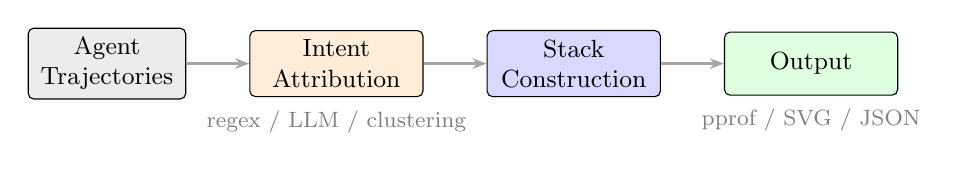
\begin{tikzpicture}[
  node distance=0.5cm and 0.8cm,
  box/.style={rectangle, draw, fill=blue!15, minimum width=2.2cm,
              minimum height=0.8cm, font=\small, align=center,
              rounded corners=2pt},
  input/.style={rectangle, draw, fill=gray!15, minimum width=2.0cm,
               minimum height=0.7cm, font=\small, align=center,
               rounded corners=2pt},
  output/.style={rectangle, draw, fill=green!12, minimum width=1.6cm,
                minimum height=0.7cm, font=\small, align=center,
                rounded corners=2pt},
  arr/.style={-{Stealth[length=1.8mm]}, thick, gray!70},
]

% Input (left)
\node[input] (traj) {Agent\\Trajectories};

% Node 1: Intent Attribution
\node[box, right=0.8cm of traj, fill=orange!15] (intent) {Intent\\Attribution};
\node[font=\footnotesize, below=0.05cm of intent, text=gray] (backends) {regex / LLM / clustering};

% Node 3: Stack Construction
\node[box, right=0.8cm of intent] (stack) {Stack\\Construction};

% Node 4: Output
\node[box, right=0.8cm of stack, fill=green!12] (out) {Output};
\node[font=\footnotesize, below=0.05cm of out, text=gray] {pprof / SVG / JSON};

% Arrows
\draw[arr] (traj) -- (intent);
\draw[arr] (intent) -- (stack);
\draw[arr] (stack) -- (out);

\end{tikzpicture}
}
\caption{Data-flow and algorithm pipeline. Local agent histories enter
through \texttt{agent-session} parsing; public datasets enter as
operation JSONL. Both paths produce uniform operations. Recursive
operation segmentation, projection, and folding are algorithms
(segmentation runs once per trajectory; projection and folding run at
query time) applied identically to both sources.}
\Description{Data-flow diagram from agent trajectories through parsing,
operation segmentation, and projection to folded-stack output.}
\label{fig:architecture}
\end{figure}

\subsection{Recursive Operation Segmentation}
% 递归 Operation 切分
\label{sec:intent}

The algorithm rests on one structural intuition: an agent's task occupies
a contiguous span of the trajectory, and it decomposes into smaller
contiguous subtasks.
% 该算法建立在一个结构直觉上：智能体的任务在轨迹上占据一段连续区间，并且可以分解为更小的连续子任务。
Task structure is therefore exactly a set of nested named intervals, and
recovering it only requires finding the transition points between them.
% 因此任务结构恰好就是一组嵌套的命名区间，恢复它只需要找到区间之间的转换点。

Because agent work has no predefined taxonomy but transitions are visible
in the content, the core algorithm is segmentation, not labeling.
% 由于智能体工作没有预定义分类法，但转换点在内容中可见，核心算法是切分而非标注。
Instead of assigning each step a class, the algorithm reads a trajectory and finds the transition points where the agent's responsibility changes.
% 算法不为每步指派类别，而是读取轨迹、找出责任变化处的转换点。
At each transition it cuts the trajectory and names the intervals on both
sides; it then recurses into each interval, cutting again wherever a
finer responsibility change remains, and stops when an interval reads as
one coherent piece of work.
% 在每个转换点它切开轨迹并为两侧的区间命名；随后对每个区间递归，在仍存在更细责任变化处继续切分，直到一个区间读起来是一件连贯的工作为止。
Formally, a trajectory is an ordered step sequence $T=(t_1,\dots,t_n)$,
and a segmentation is a set $S$ of named intervals over $T$ that is
nested (any two intervals are disjoint or one contains the other),
covers every step, and contains the whole-session interval as its root.
% 形式化地，轨迹是有序步骤序列 $T=(t_1,\dots,t_n)$；切分是 $T$ 上的命名区间集合 $S$：区间两两要么不相交、要么一个包含另一个（嵌套），共同覆盖每个步骤，且以整个 session 区间为根。
The algorithm computes $S$ by one recursive rule: $\textsc{Segment}(I)$ selects zero or more transition points inside interval $I$, which partition $I$ into consecutive child intervals; each child receives a short action-first name and is segmented recursively; selecting no transition terminates the branch.
% 算法用一条递归规则计算 $S$：$\textsc{Segment}(I)$ 在区间 $I$ 内选择零个或多个转换点，将 $I$ 划分为连续的子区间；每个子区间获得一个动词优先的短名称并被递归切分；不再选择转换点即终止该分支。
A step's operation path is the name chain of the intervals containing it, from the session root to its innermost interval; equal paths fold across sessions.
% 一个步骤的 operation 路径是包含它的区间自 session 根到最内层的名称链；相同路径跨 session 折叠。
Segmentation is the right primitive for three reasons.
% 切分是正确的基本操作，原因有三。
First, transitions are what a trajectory actually exhibits: agent work
has no predefined taxonomy, but a shift in what the agent is trying to
do is visible in the source content itself.
% 其一，转换点是轨迹真实呈现的东西：智能体工作没有预定义分类法，但"智能体正在做的事发生了变化"在源内容中是可见的。
Second, cuts compose: nested intervals form a hierarchy whose depth
emerges per branch from the content rather than from a prescribed
schema.
% 其二，切口可组合：嵌套区间构成层次，其深度按分支从内容中涌现，而非来自规定的 schema。
Third, naming intervals rather than steps yields identifiers at the
granularity where recurrence lives, so the same short action-first name
(one to three words) reappears across sessions and folds.
% 其三，为区间而非单步命名，得到与"重复出现"粒度一致的标识符——同一个动词优先的短名称（一到三个词）在不同 session 中再次出现并得以折叠。
Concretely, in one Git-deployment execution the algorithm cuts the session into \texttt{build deployment system} and, inside it, cuts again where the agent stops writing configuration and starts debugging access, yielding \texttt{deploy branches} and \texttt{diagnose authentication}; a step inside the latter carries the path \texttt{build deployment system > diagnose authentication}, and because the same names reappear in the other two executions, their costs fold together in Figure~\ref{fig:flamegraph}.
% 具体地，在一次 Git 部署执行中，算法先把 session 切为 \texttt{build deployment system}，再在"智能体从编写配置转向调试访问"处继续切分，得到 \texttt{deploy branches} 与 \texttt{diagnose authentication}；后者内部的步骤携带路径 \texttt{build deployment system > diagnose authentication}；由于同样名称在另外两次执行中再次出现，其开销在 Figure~\ref{fig:flamegraph} 中折叠到一起。
Any implementation able to find transitions and name intervals (an agent, a language model, or a statistical rule) can serve as the segmenter.
% 任何能找到 transition 并为 interval 命名的实现（agent、语言模型或统计规则）都可作为 segmenter。
In evaluation, we use Codex~\cite{codex}, invoked once per trajectory with one fixed instruction:
% 在评估中，我们使用 Codex，每条轨迹调用一次，使用固定指令：

\begin{quote}\small
\emph{Input:} one trajectory (each step's prompt, command, and output summary, with no labels or scores).\\
\emph{Action:} read it, emit a mark wherever the responsibility changes, and use \sys to check and update the segmentation, and re-read and update the marks iteratively until you think the segmentation is complete.\\
\emph{Output:} sparse path marks, e.g.,\\
{\ttfamily step 1: [deploy git server]\\
step 4: [deploy git server, diagnose SSH access]\\
step 15: [deploy git server, verify web endpoint]}\\
---one line only where the path changes; names of one to three action-first words.
\end{quote}

% 输入：一条轨迹（每步的提示词、命令与输出摘要，不含标签或分数）。动作：读取轨迹，在责任变化处发出 mark，并用 \sys 检查和更新切分，反复阅读和更新 mark 直到认为切分完整。输出：稀疏路径 mark，仅在路径变化处出现一行，名称为一到三个动词开头的词。
The sparse marks still produce a complete segmentation: steps between two marks inherit the preceding path.
% 稀疏的 mark 仍产生完整切分：两个 mark 之间的步骤继承前一条路径。
Segmentation is not a one-shot labeling pass: the agent can revise marks, refine interval names, and add deeper cuts iteratively until it judges the hierarchy complete.
% 切分不是一次性标注：agent 可以修改标记、精炼区间名称、添加更深的切分，迭代进行直到它认为层次完整为止。
Revisions are incremental: changing one interval does not require re-annotating the entire trajectory.
% 修改是增量的：改动一个区间不需要重新标注整条轨迹。
Although we evaluate segmentation offline, the model also supports online incremental annotation during agent execution.
% 虽然我们离线评估切分，但该模型也支持在 agent 执行过程中进行在线增量标注。

%% ===================================================================
\section{Implementation}
% 实现
\label{sec:impl}

\sys is implemented as a Rust CLI ({$\sim$}9.8K LOC, Figure~\ref{fig:architecture}).
% \sys 实现为 Rust CLI（约 9.8K 行代码，Figure~\ref{fig:architecture}）。
It reads Codex and Claude Code local JSONL history files and AgentSight~\cite{agentsight} recordings for system effects.
% 它读取 Codex 和 Claude Code 本地 JSONL 历史文件以及 AgentSight~\cite{agentsight} 的系统副作用记录。
The pipeline has two stages: first, preprocessing extracts a readable trajectory summary; then, the segmentation agent reads this summary and writes interval marks to an annotation file, which it can revise until satisfied.
% 管线分两阶段：首先预处理提取可读的轨迹摘要；然后切分 agent 读取摘要并将区间标记写入标注文件，它可以反复修改直到满意为止。
The CLI validates that marks are nested and cover every step, then emits a standard pprof protobuf profile that \texttt{go tool pprof} reads directly.
% CLI 校验标记嵌套且覆盖每一步，然后输出标准 pprof protobuf profile，供 \texttt{go tool pprof} 直接读取。
Projection is deterministic: each operation contributes its semantic path and LLM/tool evidence, with session identities kept as pprof labels rather than visible frames, so equal semantic prefixes fold across sessions.
% 投影是确定性的：每个 operation 提供其语义路径与 LLM/tool 证据，session 身份作为 pprof label 而非可见 frame 保留，因此相同语义前缀可跨 session 折叠。
Switching the additive measure replays the same annotations and changes only stack widths.
% 切换可加度量只重放同一标注、只改变栈宽度。

\paragraph{Annotated and literal levels.}
% 标注层级与字面层级。
A level in the operation stack need not come from annotation.
% operation stack 中的层级不必来自标注。
Any responsibility the source log already records literally can become a level directly, at no annotation cost and with no tag error, provided its extent satisfies the same interval contract.
% 只要其区间满足同一份契约，任何源日志已经字面记录的责任都可以直接成为一个层级，且不付出标注成本、不引入标签误差。
Agent skills are the concrete case: a scope opens at an exact recorded skill invocation and closes at the next invocation or the next user prompt, which keeps the intervals nested, noncrossing, and covering, so the level folds and conserves exactly like an annotated one.
% agent skill 是具体例子：作用域在一次被精确记录的 skill 调用处开启，在下一次调用或下一个用户 prompt 处关闭，从而保持区间嵌套、不交叉且全覆盖，因此该层级与标注层级一样可折叠、可精确守恒。
The two kinds compose in one stack---annotated semantic responsibility above, exact literal levels beneath it---and each literal field is also emitted as a pprof label, so stock \texttt{-tagfocus} selects the same scope a frame does.
% 两类层级组合在同一个栈中——标注得到的语义责任在上，精确的字面层级在其下——每个字面字段同时作为 pprof label 输出，因此原生 \texttt{-tagfocus} 选中的范围与 frame 一致。
Because a literal level costs nothing to construct, it extends to a developer's complete history while annotated levels cover the annotated portion of it.
% 由于字面层级的构建不产生成本，它可以覆盖开发者的完整历史，而标注层级只覆盖其中被标注的部分。

\paragraph{Non-LLM statistical segmenter.}
% 非 LLM 统计 segmenter。
The statistical segmenter scores adjacent action transitions by normalized pointwise mutual
information~\cite{bouma2009npmi} and calibrates a label-free cutoff with
occurrence-weighted two-means~\cite{macqueen1967}, treating detailed
recurrence as continuity that can remove but never add a coarse boundary.
An optional reference-calibrated mode fits one scalar cutoff on disjoint
reference groups.
% 统计 segmenter 用归一化点互信息为相邻 action 转移评分，并用按出现次数加权的二均值校准无标签阈值；detail 连续性只能删除、不能新增粗边界；可选的 reference-calibrated 模式在不重叠的参考分组上拟合单一标量阈值。

%% ===================================================================
\section{Evaluation}
% 评估
\label{sec:eval}

The evaluation addresses four research questions.
% 评估回答四个研究问题。
\textbf{RQ1:} Does semantic profiling improve resource attribution?
\textbf{RQ2:} Does profiler output correspond to real problems?
\textbf{RQ3:} How accurate are the tags?
\textbf{RQ4:} What is the profiling cost?
Together they form one chain: semantic responsibility can be recovered
accurately (RQ3), the recovered hierarchy aggregates across runs while
conserving every additive measure (RQ1), the aggregate corresponds to real
problems and reduces the evidence a reader must open (RQ2), and construction
and replay costs are measured and practical (RQ4).
% 四个 RQ 构成一条链：语义责任可以被准确恢复（RQ3）；恢复的层次跨运行聚合并精确守恒每种可加度量（RQ1）；聚合结果对应真实问题并减少 reader 必须打开的证据（RQ2）；构建与重放成本可测且实用（RQ4）。

We evaluate three data classes.
% 我们评估三类数据。
\emph{Real inputs}: 41 long-horizon coding-agent sessions (three of which
repeat one Git-deployment task and form the RQ1 case), 440 mixed-outcome
web-agent trajectories~\cite{agentrewardbench}, and one developer's complete
local session history from the authors' workstation (1{,}394 sessions), whose
42 long-horizon development sessions are the annotated portion.
% 真实输入：41 条 long-horizon coding-agent session（其中三条重复同一个 Git 部署任务，构成 RQ1 案例）、440 条 mixed-outcome web-agent 轨迹，以及作者工作站上一位开发者的完整本地 session 历史（1,394 个 session），其中 42 条 long-horizon 开发 session 是被标注的部分。
\emph{Annotated trajectories}: 405 CodeTraceBench trajectories with
20{,}866 operations and 2{,}948 human-verified
stages~\cite{li2026codetracer}, 287 OSWorld-Human
sessions~\cite{osworldhuman}, 1{,}012 AgentBoard goals~\cite{agentboard},
and 2{,}737 published action
labels~\cite{bouzenia-pradel-2025-trajectories}.
% 标注轨迹：405 条 CodeTraceBench 轨迹（20,866 个 operation、2,948 个人工核验 stage）、287 个 OSWorld-Human session、1,012 个 AgentBoard goal 与 2,737 个公开 action 标签。
\emph{Problem-localization benchmarks}: the complete AgentProcessBench,
HINTBench, and TraceElephant workloads, where every trajectory carries an
independently annotated faulty step, over 27{,}346
operations~\cite{agentprocessbench,hintbench,traceelephant}.
% 问题定位 benchmark：完整的 AgentProcessBench、HINTBench 与 TraceElephant workload——每条轨迹带有独立标注的出错步骤——共 27,346 个 operation。
All annotations, outcomes, and scores stay hidden from every method
until its output is frozen.
% 所有标注、结局与分数在每个方法的输出冻结之前都对其保持隐藏。
Mean operations per trajectory are 8.5 (AgentProcessBench), 13.9
(OSWorld-Human), 24.0 (HINTBench), 27.1 (TraceElephant), and 51.5
(CodeTraceBench), so the benchmark trajectories are short-to-medium horizon
while the annotated 42-session workstation portion---whose longest sessions
span tens of hours---supplies the long-horizon regime; the RQ4 union covers
27{,}765 operations.
% 各 workload 平均每条轨迹的 operation 数分别为 AgentProcessBench 8.5、OSWorld-Human 13.9、HINTBench 24.0、TraceElephant 27.1、CodeTraceBench 51.5，因此 benchmark 轨迹属于短到中 horizon，而被标注的 42-session 工作站部分（最长 session 跨越数十小时）提供长 horizon 区间；RQ4 的并集覆盖 27,765 个 operation。

%% -------------------------------------------------------------------
\subsection{RQ1: Does Semantic Profiling Improve Resource Attribution?}
% RQ1：语义 profiling 是否改善资源归因？

\emph{Setup.} We test one necessary consequence of the claim: whether a fixed
semantic hierarchy reveals materially different bottlenecks when the additive
resource measure changes.
% 设置。我们检验该主张的一个必要后果：固定的语义层次在切换可加资源度量时是否暴露实质不同的瓶颈。
The population contains 41 real long-horizon agent trajectories and 5{,}750 operations, including three independent executions of one Git-deployment task with 96 recursive annotations.
% population 含 41 条真实 long-horizon agent 轨迹与 5,750 个 operation，其中包含同一 Git 部署任务的三次独立执行，共 96 个递归标注。
The resulting hierarchy reaches semantic depth five without a fixed limit.
% 所得层次在无固定上限下达到语义深度五。

\paragraph{The motivating case revisited.}
% 动机案例回顾。
The Git-deployment case from Section~\ref{sec:background} established that semantic organization reunites cross-run responsibility that native and coarse organizations scatter.
% 第~\ref{sec:background} 节的 Git 部署案例建立了语义组织能重聚跨运行责任、而 native 和 coarse 组织会将其分散。
Here we add a third measure: elapsed time.
% 这里我们增加第三种度量：elapsed time。
The same hierarchy replays under all three measures with exact conservation, and the \texttt{diagnose authentication} subtree's share rises from 21\% (count) through 37\% (time) to 46\% (tokens)---changing only the measure moves the attributed share by more than a factor of two.
% 同一层次在三种度量下精确守恒地重放，\texttt{diagnose authentication} 子树的份额从 21\%（count）经 37\%（time）升至 46\%（token）——仅改变度量就使归因份额变化超过两倍。
A quantitative control shows why alternative organizations fail: of 105 authentication operations, 102 carry only the raw-action label \texttt{run}, and that same \texttt{run} bucket mixes in 97 unrelated operations; coarse action-kind scatters the work across six categories (execute 39\%, version-control 22\%, edit 19\%, inspect 12\%, search 7\%, install 1\%); native call trees place each operation under a distinct source call with no shared responsibility node.
Only the semantic hierarchy reunites authentication into one focusable cross-run path while preserving all call/tool evidence as drilldown leaves.
% 定量对照显示为什么其他组织方式失败：105 个认证 operation 中 102 个只带 raw-action 标签 \texttt{run}，而同一个 \texttt{run} bucket 还混入 97 个无关 operation；coarse action-kind 把工作散落到六个类别（execute 39\%、version-control 22\%、edit 19\%、inspect 12\%、search 7\%、install 1\%）；native call tree 把每个 operation 放在不同 source call 下，没有共享责任节点。只有语义层次将认证重聚为一条可聚焦的跨运行路径，同时保留所有 call/tool 证据作为下钻叶。
Separately, real AgentSight~\cite{agentsight} eBPF recordings replay the
same way: the R114 population folds all 1{,}520 process and file effects
under task responsibilities through the recorded wrapper tool with exact
conservation, demonstrating the system-effect layer end to end.
% 此外，真实的 AgentSight eBPF recording 以相同方式重放：R114 population 通过记录的 wrapper tool，把全部 1,520 个 process 与 file effect 精确守恒地折叠到 task responsibility 之下，端到端展示了 system-effect 层。

\paragraph{Use case 2: where did this project's agent budget go?}
% 用例 2：这个项目的 agent 预算去哪了？
A developer spent weeks building \sys{} and this paper with coding agents, accumulating a local session history whose long-horizon portion---42 sessions (18 Codex, 24 Claude Code), 1{,}252 prompts, 5{,}620 LLM calls, and 1.38 billion tokens---is annotated here.
% 一位开发者花数周用 coding agent 构建 \sys{} 与本文，累积了一份本地 session 历史，这里标注的是其中的 long-horizon 部分——42 个 session（18 Codex、24 Claude Code）、1,252 个 prompt、5,620 次 LLM 调用和 13.8 亿 token。
The question: \emph{what did the agents actually spend tokens doing?}
% 问题：agent 到底把 token 花在了什么事上？
The profile (Figure~\ref{fig:selfprofile}) shows the answer is not one dominant sink but a broad distribution: the largest path (\texttt{refine paper > align evaluation}) holds only 1.7\% of tokens.
% profile（Figure~\ref{fig:selfprofile}）显示答案不是单一大头而是宽分布：最大路径（\texttt{refine paper > align evaluation}）仅占 1.7\% 的 token。
The three longest sessions (spanning tens of hours each) keep distinct dominant responsibilities (evaluation alignment, evidence inspection, and merge resolution), so session structure is preserved rather than averaged away.
% 三条最长 session（各跨越数十小时）各有不同的主导责任（evaluation alignment、evidence inspection、merge resolution），session 结构被保留而非被平均抹掉。
Switching to operation count shifts where mass concentrates: token mass stays at prompt depth (70\%), while operation mass resolves deeper (44\% at depths three and four) exactly where repeated engineering work concentrates.
% 切换到 operation 数改变了质量集中处：token 质量停在 prompt 深度（70\%），而 operation 质量解析更深（44\% 在深度三和四），恰在重复工程工作集中处。

\begin{figure*}[t]
\centering
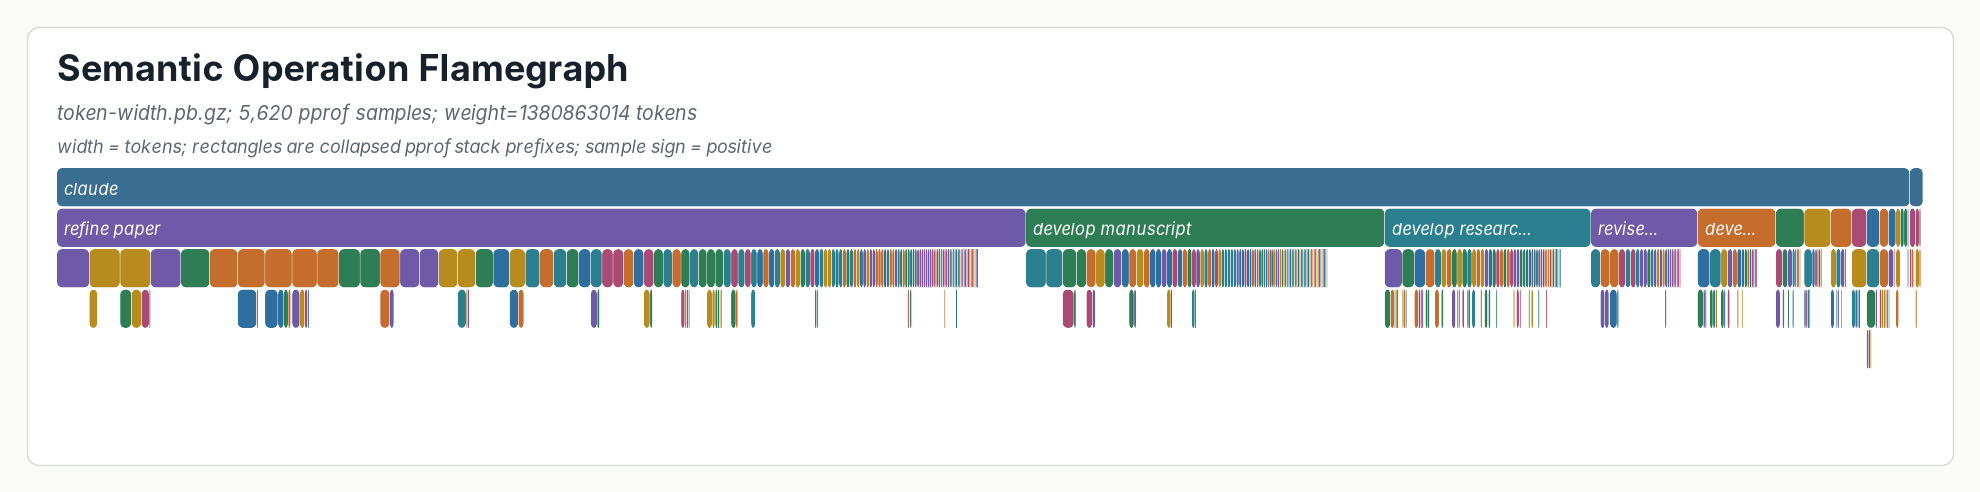
\includegraphics[width=.97\linewidth]{figures/selfprofile.tokens.png}\\[1pt]
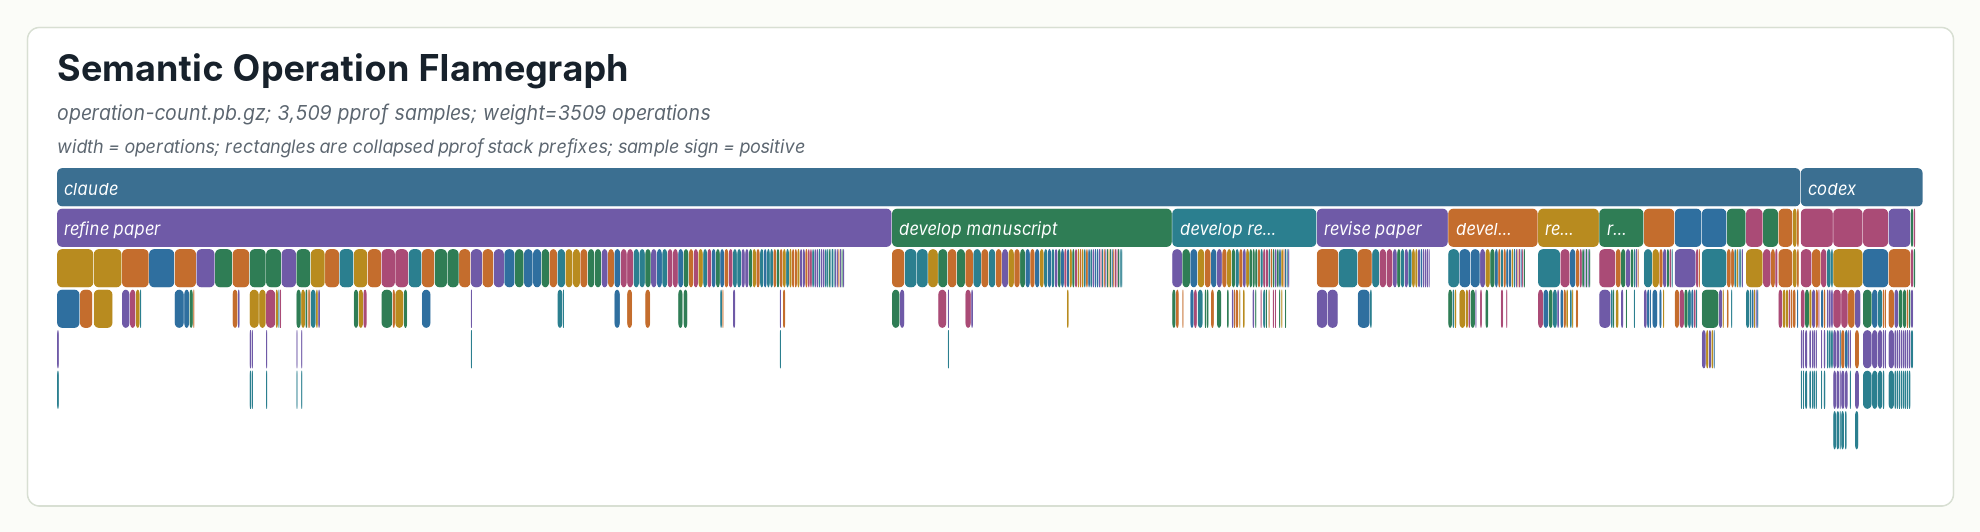
\includegraphics[width=.97\linewidth]{figures/selfprofile.operations.png}
\caption{The 42-session population under one fixed semantic hierarchy.
Width is tokens (top) or operation count (bottom); second-level frames are
annotated responsibilities (\texttt{refine paper}, \texttt{develop manuscript},
...), with deeper refinements available for drilldown in stock pprof.}
\Description{Two flame graphs over the same 42 development sessions. Both
show a claude root spanning most width, semantic responsibilities at the
second level, and fragmented deeper refinements.}
\label{fig:selfprofile}
\end{figure*}

The same hierarchy replays under FILE-READ, FILE-WRITE, and NETWORK-target
widths with exact conservation of 737, 31, and 61 target references
(Figure~\ref{fig:selfprofile-write}); in the FILE-WRITE view, each created
file appears as an exact drilldown leaf beneath the operation that created
it.
% 同一层次还按 FILE-READ、FILE-WRITE 与 NETWORK-target 宽度重放，分别精确守恒 737、31 与 61 个 target reference（Figure~\ref{fig:selfprofile-write}）；在 FILE-WRITE 视图中，每个被创建的文件作为精确下钻叶出现在创建它的 operation 之下。
These views ground the Introduction's system-effect question at the
substrate level: every recorded file and network target is attributed to
the semantic responsibility that touched it, making side effects auditable
per responsibility.
% 这些视图把 Introduction 的 system-effect 问题落到基底层面：每个被记录的 file 与 network target 都归因到触及它的语义责任，使副作用可按责任审计。

\begin{figure*}[t]
\centering
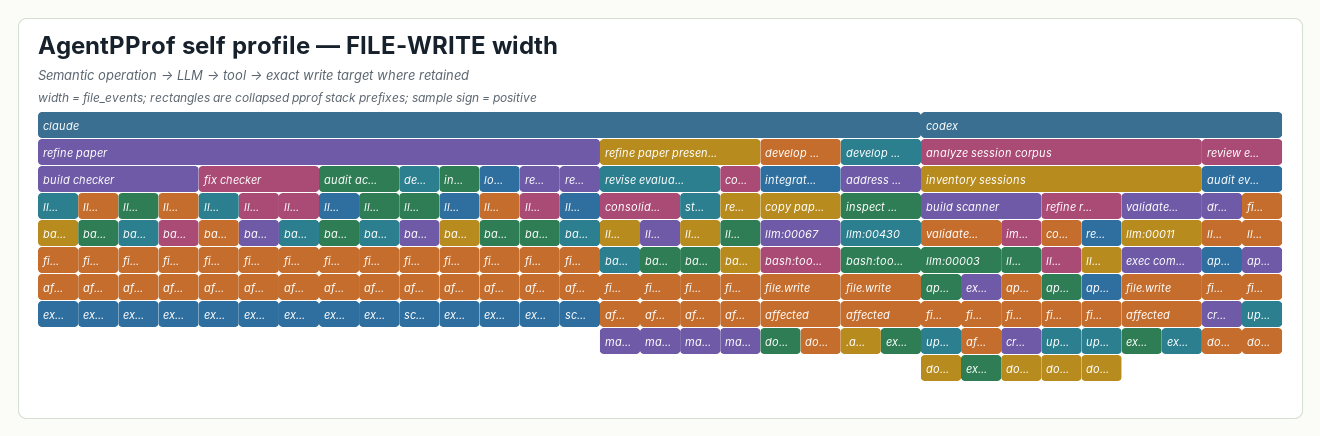
\includegraphics[width=.97\linewidth]{figures/selfprofile.file-write.png}
\caption{FILE-WRITE view of the same hierarchy: width is write count, with each created file preserved as a drilldown leaf.}
\Description{A FILE-WRITE flame graph whose semantic-operation frames contain LLM and tool frames ending at exact file-write targets.}
\label{fig:selfprofile-write}
\end{figure*}
Not every level requires annotation.
% 并非每一层都需要标注。
Skill invocations appear literally in the session log, so that level costs no
annotation time and carries no tag error, and it therefore covers the
developer's complete history rather than only its annotated portion:
1{,}394 sessions and 6{,}890{,}216{,}049 tokens.
% skill 调用在 session log 中被字面记录，因此该层级不消耗标注时间、不引入标签误差，可以覆盖开发者的完整历史而不只是其中被标注的部分：1,394 个 session 与 6,890,216,049 个 token。
A skill scope opens at an exact recorded invocation and closes at the next
invocation or the next user prompt, which keeps the intervals nested,
noncrossing, and covering, and the level conserves exactly.
% 一个 skill 作用域在被精确记录的调用处开启、在下一次调用或下一个用户 prompt 处关闭，从而保持区间嵌套、不交叉且全覆盖，该层级精确守恒。
Under it, \texttt{paper-writing-style} leads by both measures---29{,}143{,}650
tokens and 523 operations over 20 sessions and 37 invocations---and 99.47\% of
its tokens are cache reads, naming its repeated-context workflow as the first
thing to inspect.
% 在该层级下，\texttt{paper-writing-style} 在两种度量上都居首——横跨 20 个 session、37 次调用，计 29,143,650 个 token 与 523 个 operation——且其 99.47\% 的 token 为 cache read，从而指出它反复拉长上下文的工作流是首先该检查的对象。
The largest single session holds only 31.23\% of that mass, so the
history-wide priority appears only after folding.
% 最大的单个 session 仅持有该质量的 31.23\%，因此这一覆盖全历史的优先级只有在折叠之后才显现。

\emph{Takeaway.} One hierarchy attributes multiple resources with exact conservation; switching measures reveals bottlenecks that operation count alone would hide, and levels recovered from annotation and from literal source fields compose in the same stack.
% 要点。同一层次精确守恒地归因多种资源；切换度量暴露出仅靠 operation 数会掩盖的瓶颈；由标注恢复的层级与来自源字段的字面层级组合在同一个栈中。


%% -------------------------------------------------------------------
\subsection{RQ2: Does Profiler Output Correspond to Real Problems?}
% RQ2：分析器输出是否对应真实问题？

RQ2 asks whether profiler output---constructed without seeing the ground-truth fault annotations---corresponds to independently annotated real problems. We answer at three levels: a differential analysis over 440 runs whose recovery signal matches expert looping labels, a localization test on three complete benchmarks, and a reading study measuring how much evidence a human must open.
% RQ2 问 profiler 输出（构建时不接触真实故障标注）是否对应独立标注的真实问题。我们在三个层次上回答：440 次运行的差分分析（其 recovery 信号对应专家 looping 标注）、三个完整 benchmark 上的定位测试，以及测量人类需要打开多少证据的阅读研究。

\begin{figure*}[!t]
\centering
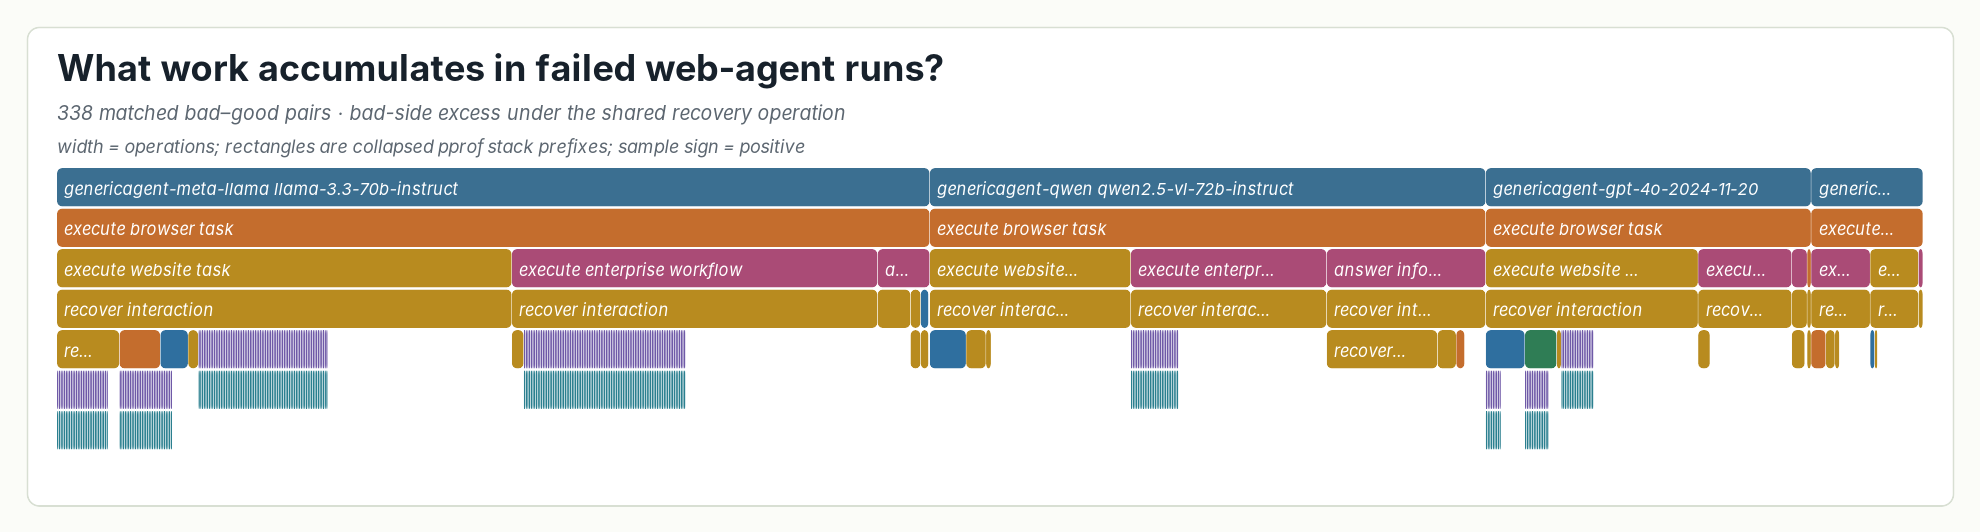
\includegraphics[width=.70\linewidth]{figures/agentreward-recovery-bad-excess.operations.png}\\[1pt]
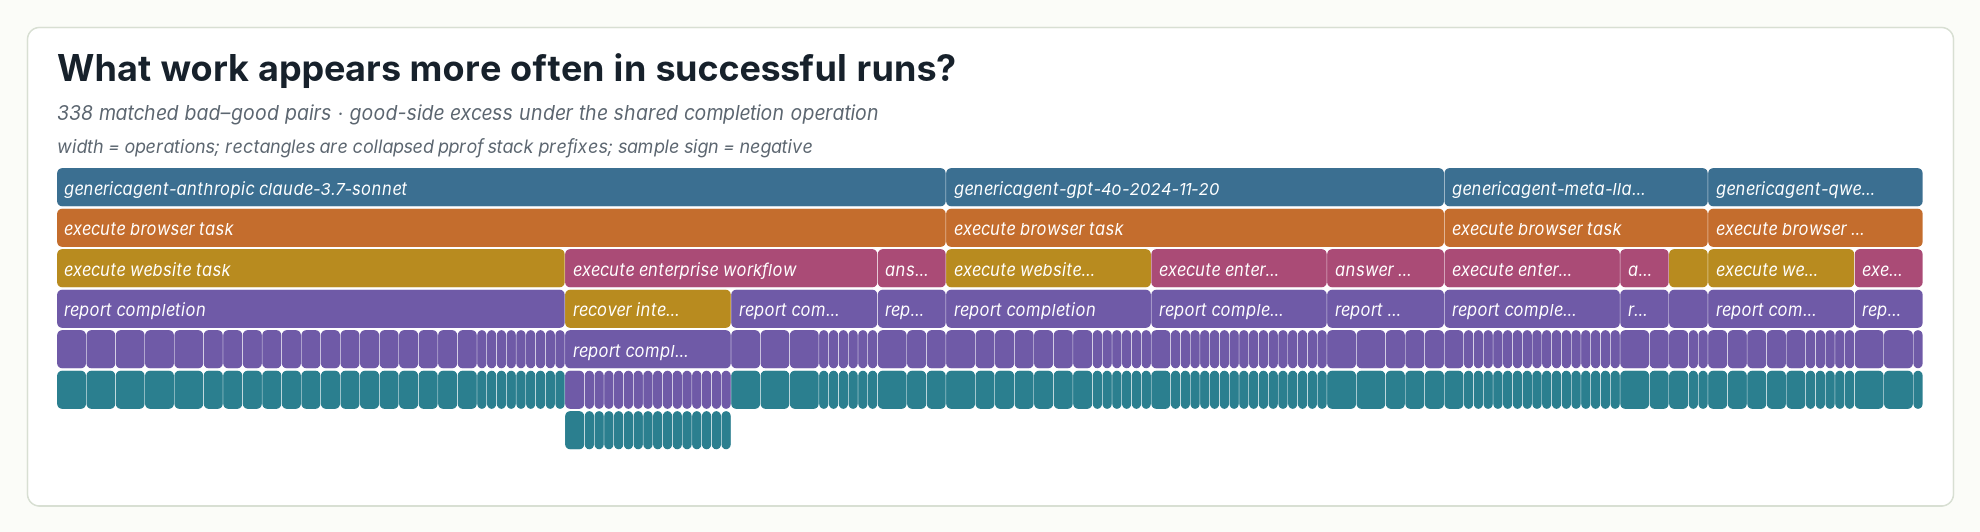
\includegraphics[width=.70\linewidth]{figures/agentreward-completion-good-excess.operations.png}
\caption{One signed profile over all 338 bad--good pairs, read from both
sides. The signed profile is the difference of two nonnegative profiles,
bad minus good, which stock pprof renders as positive and negative sample
values. \emph{Top:} positive samples under \texttt{recover interaction},
3{,}286 bad-side versus 455 good-side occurrences. \emph{Bottom:} negative
samples under \texttt{report completion}, 135 bad-side versus 191 good-side
occurrences. These are aggregate diagnostic differences, not causal
effects.}
\Description{Two flame graphs of a signed difference profile. The upper
graph descends from browser-task responsibilities into recovery work and
specific retry, search, and inspection operations. The lower graph descends
through task completion into its source LLM and tool calls.}
\label{fig:diff-flamegraph}
\end{figure*}

\paragraph{Use case 3: what do failing runs do differently?}
% 用例 3：失败的运行到底做了什么不同？
A team has 440 web-agent runs~\cite{agentrewardbench} over 125 tasks, where every task has both successful and failed attempts (202 successful, 238 failed).
% 一个团队有 125 个任务的 440 次 web-agent 运行（202 成功、238 失败），每个任务都同时有成功与失败的尝试。
The question: \emph{what behavior separates success from failure?}
% 问题：什么行为区分成功与失败？
Reading 440 transcripts (7{,}229 operations) is infeasible.
% 阅读 440 份转录（7,229 个 operation）不现实。
A signed difference profile (bad minus good, Figure~\ref{fig:diff-flamegraph}) answers at a glance: failed runs spend 45\% of their steps in \texttt{recover interaction} (retrying, re-searching, re-navigating) versus only 12\% for successful runs.
% 带符号差分 profile（bad 减 good，Figure~\ref{fig:diff-flamegraph}）一眼给出答案：失败运行花 45\% 的步骤在 \texttt{recover interaction}（重试、重搜索、重导航），而成功运行只有 12\%。
Drilldown decomposes the recovery responsibility into verification challenges, repeated searches, mistaken navigation, and record retries, with source labels identifying which sessions contributed each width.
% 下钻把 recovery 责任分解为验证挑战、重复搜索、误导航和记录重试，source label 指明哪些 session 贡献了各宽度。
The insight: failing agents get stuck in retry loops rather than backing out and trying a different approach.
% 洞察：失败的 agent 陷入重试循环，而不是回退尝试不同方法。
This structure matches independent expert looping labels at AP 0.63 (baseline 0.40), confirming the profile surfaces a real behavioral pattern, not an artifact of step count.
% 该结构与独立专家 looping 标注的一致性为 AP 0.63（基线 0.40），确认 profile 呈现的是真实行为模式而非步骤数的副产物。

\paragraph{Supplementing benchmark-native diagnostics.}
% 补充 benchmark 原生诊断。
\emph{Setup.} Each benchmark trajectory has one annotated faulty step;
a method outputs a ranking of that trajectory's operations, scored by
average precision (AP approximates the reciprocal rank of the faulty step) and
averaged as MAP~\cite{robertson2008ap}.
% 设置。每条 benchmark 轨迹有一个已标注的出错步骤；方法输出对该轨迹 operation 的排序，以 average precision 评分（单目标时 AP 约等于出错步骤排名的倒数），并平均为 MAP。
We run the complete AgentProcessBench, HINTBench (the complete released test
snapshot, 536 of the paper-reported 629 trajectories), and TraceElephant
workloads; operations, target-blind paths, benchmark predictions, and scoring
are fixed before test targets are loaded.
% 我们在完整的 AgentProcessBench、HINTBench（完整的已发布 test snapshot，即论文报告的 629 条中的 536 条）与 TraceElephant workload 上运行；operation、target-blind path、benchmark 预测与评分规则都在加载 test target 之前固定。
Each query is one trajectory containing an annotated target, and we report
non-interpolated per-query AP averaged over 614, 400, and 220 target-bearing
queries; all 522 zero-positive trajectories are consumed for population
coverage but excluded from MAP because AP is undefined without a relevant
item.
% 每个 query 是一条含标注 target 的轨迹，我们报告未插值的 per-query AP，并在 614、400 与 220 个带 target 的 query 上取算术平均；全部 522 条 zero-positive 轨迹计入群体覆盖，但因缺少相关项使 AP 无定义而从 MAP 中排除。
The \emph{direct diagnostic} is the per-operation output of a
benchmark-native process judge (AgentProcessBench risk units) or trajectory
localizer (HINTBench, TraceElephant), which for TraceElephant reads the full
trace and reference answer before naming the responsible agent and decisive
step.
% \emph{direct diagnostic} 是 benchmark 原生 process judge（AgentProcessBench 的 risk unit）或 trajectory localizer（HINTBench、TraceElephant）的逐 operation 输出；在 TraceElephant 上，它先读取完整 trace 与参考答案，再指出责任 agent 与决定性步骤。
\emph{Direct-only} ranks by that diagnostic alone; \emph{Direct+AgentProf}
ranks lexicographically by (direct diagnostic, target-blind group score) and
can therefore only refine exact diagnostic-score ties;
\emph{Direct+\sys-Raw} is the information-matched ablation of \sys that
groups by raw action instead of semantic names, with identical source-kind,
tool/call, and outcome suffix and aggregation; \emph{AgentProf-only} drops
the benchmark diagnostic (Table~\ref{tab:rq2-localization}).
% Direct-only 仅按该诊断排序；Direct+AgentProf 按 (direct diagnostic, target-blind 组分数) 的字典序排序，因此只能细化诊断分数完全并列的情形；Direct+\sys-Raw 是 \sys 的信息量匹配消融，按 raw action 而非语义名分组，并保留完全相同的 source-kind、tool/call、outcome 后缀与聚合方式；AgentProf-only 则不使用 benchmark 诊断（Table~\ref{tab:rq2-localization}）。

\begin{table}[tb]
\centering\small
\setlength{\tabcolsep}{1.8pt}
\begin{tabular}{@{}lrrrr@{}}
\toprule
Workload & \shortstack{Direct+\\\sys} & \shortstack{Direct+\\\sys-Raw} & \shortstack{Direct\\only} & \shortstack{\sys\\only} \\
\midrule
AgentProcessBench & \textbf{.894} & \textbf{.893} & .863 & .791 \\
HINTBench & \textbf{.517} & \textbf{.518} & .411 & .432 \\
TraceElephant & \textbf{.326} & \textbf{.324} & .209 & .259 \\
\bottomrule
\end{tabular}
\caption{MAP over the complete RQ2 populations (614, 400, and 220
target-bearing queries). \sys-Raw ablates only \sys's semantic prefix; bold
marks each workload's best methods. Higher is better.}
\label{tab:rq2-localization}
\end{table}

\begin{figure}[tb]
\centering
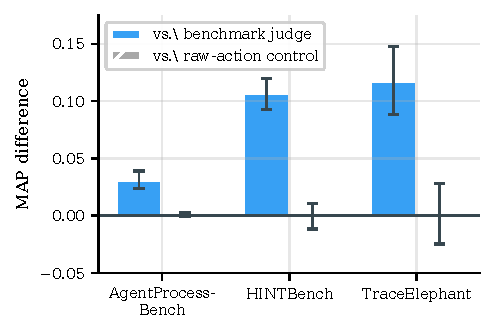
\includegraphics[width=\columnwidth]{figures/fig-rq2-deltas.pdf}
\caption{Paired MAP differences over the complete RQ2 populations, with 95\%
intervals from 10{,}000 trajectory-cluster resamples of unrounded per-query
APs. Adding the target-blind profile to each benchmark's own judge improves
ranking on all three workloads (left bars, intervals entirely above zero),
whereas the semantic prefix and the information-matched \sys-Raw ablation
are indistinguishable (right bars, intervals spanning zero). Grouping plus
retained evidence, not the semantic names, drives this gain.}
\Description{A grouped bar chart of MAP differences on three workloads. The
bars comparing the profile-refined ranking against the benchmark judge are
positive on all three workloads with error bars above zero, while the bars
comparing the semantic prefix against the raw-action ablation sit at zero with
error bars crossing it.}
\label{fig:rq2-deltas}
\end{figure}

\emph{Results.} Direct+AgentProf beats Direct-only by 0.031 [0.024, 0.039],
0.107 [0.093, 0.120], and 0.117 [0.088, 0.148], using 10{,}000 paired resamples of
trajectory clusters within benchmark-defined strata, so every paired interval
lies above zero (Figure~\ref{fig:rq2-deltas}).
% 结果。Direct+AgentProf 相对 Direct-only 分别提高 .031 [.024,.039]、.107 [.093,.120] 与 .117 [.088,.148]（在 benchmark 定义的分层内对轨迹簇做 10,000 次配对重抽样），因此每个配对区间都位于零以上。
The semantic and \sys-Raw refinements reach the same ranking quality
(.893, .518, and .324), confirming that grouping plus retained
evidence---not naming alone---drives the localization gain over Direct-only.
% 语义与 \sys-Raw 两种细化达到相同的排序质量（.893、.518 与 .324），确认了"分组+保留的证据"（而非单独的命名）驱动相对 Direct-only 的定位增益。
The semantic prefix earns its value in two other measured roles:
cross-run attribution (RQ1) and directing a reader's attention, which the
following study measures.
% 语义前缀另有两个独立测量的作用：跨运行归因（RQ1）与引导读者的注意力，后者由下面的研究测量。

\paragraph{Profile-guided reading on TraceElephant.}
% TraceElephant 上的 profile 引导阅读。
On the complete 220 queries that contain a faulty step, a Grok~4.5~\cite{grok45} agent receives the task description and trajectory content (without any ground-truth labels) and is asked to rank operations by likely fault; operations appear in original order with one agent invocation per stage.
% 在全部 220 个含出错步骤的 query 上，Grok 4.5 agent 接收任务描述与轨迹内容（不含任何真实标签），被要求按可能出错排序 operation；operation 按原始顺序呈现，每阶段一次 agent 调用。
Full-trace reading reaches MAP .502 at a mean 12{,}615 input tokens per
query, versus .209 for the benchmark's Direct-only diagnostic and .326 for
Direct+AgentProf.
% 全 trace 阅读以每 query 平均 12,615 个输入 token 达到 MAP .502，而 benchmark 的 Direct-only 诊断为 .209、Direct+AgentProf 为 .326。
A two-stage profile-guided variant first shows only the semantic operation
skeleton, with no source content, and the reader selects at most five groups;
stage two then opens only those groups' evidence.
% 两阶段的 profile 引导变体先只展示语义 operation 骨架（不含 source 内容），reader 最多选择五个 group；第二阶段只打开这些 group 的证据。
It reaches MAP .455 while opening 53.0\% of the source content, and its
stage-one selections never fell back to a default: the five-group budget
saturated on 99.5\% of queries, re-parsing the uncapped stage-one responses
shows the reader proposed more than five groups on zero of 220 queries, and
every missed target group was entirely absent from its ordered selection
rather than cut off by the budget.
% 它在只打开 53.0\% source 内容的情况下达到 MAP .455，且第一阶段的选择从未回退到默认值：五组预算在 99.5\% 的 query 上被用满；重新解析未截断的第一阶段响应显示，reader 在 220 个 query 中的 0 个上提出了超过五组；每个被遗漏的 target group 都是整体缺席于其有序选择，而非被预算截断。
Under the information-matched \sys-Raw skeleton, ranking quality is
statistically unchanged (MAP .465; paired delta $+.010$ [$-.021$, $+.042$]),
but the reader opens significantly more content: 65.0\% versus 53.0\%, paired
delta $+.120$ [$+.103$, $+.137$], and $2.80$ [$1.96$, $3.60$] more evidence
operations.
% 在信息量匹配的 \sys-Raw 骨架下，排序质量在统计上不变（MAP .465；配对差 +.010 [-.021,+.042]），但 reader 打开的内容显著更多：65.0\% 对 53.0\%，配对差 +.120 [+.103,+.137]，且多打开 2.80 [1.96,3.60] 个 evidence operation。
Semantic naming's measured contribution in this regime is therefore
attention concentration at equal quality.
% 因此在该机制下，语义命名可测得的贡献是"同等质量下的注意力集中"。
A per-query full read is also bounded by the model context window (the
4{,}558{,}192-token Git population cannot be read whole), whereas
skeleton-guided reading stays available at any trace length once the profile
exists. The reader is query-specific while the hierarchy is constructed
once and replayed across queries and measures.
% 每 query 的全量阅读还受模型上下文窗口约束——4,558,192-token 的 Git population 无法整体读入——而骨架引导的阅读在 profile 存在后对任意 trace 长度都可用；此外 reader 是 query-specific 的，而层次只构造一次并跨 query 与度量重放。
\emph{Takeaway.} Failure structure surfaced by the profile matches
independent human labels at collection scale; profiles add localization
signal on top of existing judges; and the semantic names buy evidence
efficiency rather than ranking accuracy.
% 要点。profile 呈现的失败结构在集合尺度上与独立人工标注一致；profile 在既有 judge 之上补充定位信号；语义名称换来的是证据效率而非排序精度。

%% -------------------------------------------------------------------
\subsection{RQ3: How Accurate Are the Tags?}
% RQ3：标签有多准确？

RQ3 asks whether recursive segmentation recovers task structure that humans would recognize.
% RQ3 问递归切分是否恢复出人类会认可的任务结构。

\emph{Setup.} Gold structure is the 2{,}948 human-verified stages over
all 405 CodeTraceBench trajectories. B$^3$
F1~\cite{bagga-baldwin-1998-entity-based} asks whether operations that
belong together end up grouped together; exact adjacent-boundary
F1~\cite{ruokolainen2016segmentation} asks whether cuts land exactly
where humans cut. Baselines receive identical inputs
(Table~\ref{tab:rq3-codetrace}).
% 设置。黄金结构是全部 405 条 CodeTraceBench 轨迹上的 2,948 个人工核验 stage。B$^3$ F1 度量"应当在一起的 operation 是否被分到一起"；精确相邻边界 F1 度量"切点是否恰好落在人工切点处"。基线获得完全相同的输入（Table~\ref{tab:rq3-codetrace}）。
Each method output is evaluated at the level it predicts: literal names by
accuracy and macro-F1~\cite{lewis2004rcv1}, permutation-invariant partitions
by V-measure~\cite{rosenberg-hirschberg-2007-v-measure} or ordinary B$^3$,
and adjacent interval boundaries by exact precision, recall, and F1; for
legacy field-valued datasets a conversion step maps each predicted
group into the same interval-annotation format before \sys folds the
original additive weights.
% 每个方法的输出按其预测的层级评估：字面名称用 accuracy 与 macro-F1，置换不变的 partition 用 V-measure 或普通 B$^3$，相邻区间边界用精确的 precision、recall 与 F1；对字段值型的既有数据集，转换步骤先把每个预测 group 映射为同一份区间标注格式，再由 \sys 折叠原始可加权重。
Codex~\cite{codex} with GPT-5.6-sol-high receives each trajectory (prompts, commands, and output summaries, with no labels or scores visible) and emits sparse interval marks over 17{,}148 steps without access to official stage annotations: 4{,}496 marks at semantic depth one (3), two (2{,}873), three (1{,}588), or four (32), with no prompt requesting a specific depth.
% Codex 配合 GPT-5.6-sol-high 接收轨迹（提示词、命令与输出摘要，不含标签或分数），在 17,148 个步骤上发出稀疏区间标记，不接触官方 stage 标注：共 4,496 个标记，语义深度为一层（3 个）、两层（2,873 个）、三层（1,588 个）与四层（32 个），且没有任何 prompt 指定深度。
Name normalization then maps the 3{,}895 free-form interval names to 783 stable short names (e.g., \texttt{diagnose authentication}); identical names across sessions merge so that recurring work folds in the final profile.
% 名称归一化把 3,895 个自由形式的区间名映射为 783 个稳定短名称（如 \texttt{diagnose authentication}）；跨 session 的相同名称合并，使重复工作在最终 profile 中折叠。

\begin{table}[tb]
\centering\small
\setlength{\tabcolsep}{2.0pt}
\begin{tabular}{@{}lrrrr@{}}
\toprule
Method & B$^3$ P & B$^3$ R & B$^3$ F1 & Bound. F1 \\
\midrule
Codex segmentation & 0.793 & 0.736 & \textbf{0.764} & \textbf{0.480} \\
Multi-resolution recurrence & 0.782 & 0.575 & 0.663 & 0.266 \\
Causal Qwen2.5-3B task stack & 0.557 & 0.792 & 0.650 & 0.257 \\
Raw-action grouping & 0.891 & 0.388 & 0.541 & --- \\
Native source tree & 0.975 & 0.249 & 0.397 & 0.259 \\
Source-native step & 0.983 & 0.221 & 0.361 & 0.246 \\
\bottomrule
\end{tabular}
\caption{Agreement with human stages on all 405 CodeTraceBench
trajectories. Causal Qwen2.5-3B is a stateful per-turn baseline that makes push/replace/stay/pop decisions.}
\label{tab:rq3-codetrace}
\end{table}

\emph{Results.} Codex segmentation reaches 0.764 B$^3$ F1 and 0.480
boundary F1, beating the strongest automatic baseline (multi-resolution recurrence) by +0.101
[0.087, 0.116] and +0.214 [0.193, 0.235] (paired task-cluster
intervals).
A stateful per-turn Qwen2.5-3B baseline that makes push/replace/stay/pop decisions reaches 0.650 B$^3$ F1 and 0.257 boundary F1, confirming that smaller models with carefully designed interfaces can produce meaningful segmentation, though Codex still leads by a substantial margin.
The marks conserve exactly 20{,}866 operations and
494{,}862{,}929 tokens.
% 结果。Codex 切分达到 0.764 B$^3$ F1 与 0.480 边界 F1，以 +0.101 [0.087,0.116] 与 +0.214 [0.193,0.235] 的配对任务簇区间超过最强自动基线（multi-resolution recurrence）。一个有状态的 per-turn Qwen2.5-3B baseline（做 push/replace/stay/pop 决策）达到 0.650 B$^3$ F1 与 0.257 边界 F1，确认较小模型配合精心设计的接口可以产生有意义的切分，尽管 Codex 仍以较大优势领先。标记精确守恒 20,866 个 operation 与 494,862,929 个 token。
Predicted groups remain largely pure subsets of gold stages
(B$^3$ precision 0.793): when segmentation disagrees with human stages,
it subdivides work rather than merging unrelated responsibilities,
preserving per-group coherence for downstream drilldown.
% 预测 group 仍是 gold stage 中较纯的子集（B$^3$ precision 0.793）：当切分与人工 stage 不一致时，它是把工作细分而非合并无关责任，从而为下游下钻保留每个 group 的连贯性。
The interface generalizes across method families: on 287 OSWorld-Human
sessions a supervised boundary predictor~\cite{mccallum-nigam-1998}
reaches 0.739 boundary F1 / 0.816 B$^3$ F1 and the no-LLM recurrence
segmenter 0.680 / 0.786 (strongest control: 0.645 / 0.678), and a target-blind
TF-IDF/K-Means method reaches V-measure 0.557 on nine Mind2Web sessions and
0.815 on 100 ScienceWorld sessions~\cite{mind2web,scienceworld}.
% 该接口在不同方法家族间泛化：在 287 个 OSWorld-Human session 上，监督边界预测器达到 0.739 边界 F1 / 0.816 B$^3$ F1，无 LLM 的 recurrence segmenter 为 0.680 / 0.786（最强对照 0.645 / 0.678）；target-blind 的 TF-IDF/K-Means 方法在 9 个 Mind2Web session 上 V-measure 为 0.557，在 100 个 ScienceWorld session 上为 0.815。
When the same instruction is frozen and transferred to OSWorld-Human via Codex with GPT-5.6-sol without adaptation, it reaches only 0.448 B$^3$ F1 and 0.149 boundary F1, predicting 569 groups for 2{,}042 gold groups---severe under-segmentation that shows cross-population generalization remains a limitation.
% 当同一 instruction 冻结后通过 Codex + GPT-5.6-sol 不经调整迁移到 OSWorld-Human 时，只达到 0.448 B$^3$ F1 与 0.149 边界 F1，对 2,042 个 gold group 预测 569 个——严重欠切分，表明跨 population 泛化仍是局限。
For closed-label literal tags, a fixed evaluation-only
Qwen3.6-27B~\cite{qwen36} classifier labels all 1{,}012 AgentBoard
goals~\cite{agentboard} into nine task families at 0.695 macro-F1 and 0.733
accuracy (majority baseline 0.044 / 0.248), and the same model
classifies all 2{,}737 published action labels from 120 AutoCodeRover,
OpenHands, and RepairAgent
trajectories~\cite{traceview-2026,bouzenia-pradel-2025-trajectories} at 0.498
macro-F1 and 0.628 accuracy (majority baseline 0.061 / 0.323).
% 在闭标签的字面标签上，固定的、仅用于评测的 Qwen3.6-27B 方法把全部 1,012 个 AgentBoard goal 分入九个 task family，macro-F1 与 accuracy 为 0.695 / 0.733（majority 基线 0.044 / 0.248）；同一模型把来自 120 条 AutoCodeRover、OpenHands 与 RepairAgent 轨迹的全部 2,737 个公开 action 标签分类，macro-F1 与 accuracy 为 0.498 / 0.628（majority 基线 0.061 / 0.323）。
\emph{Takeaway.} Recursive segmentation is the most accurate tested
automatic constructor on both structural axes, and non-LLM methods
implementing the same interface remain viable when no model is available.
% 要点。递归切分是两个结构轴上最准确的被测自动构造器；实现同一接口的非 LLM 方法在没有模型可用时依然可行。

%% -------------------------------------------------------------------
\subsection{RQ4: What Is the Profiling Cost?}
% RQ4：分析开销是多少？

RQ4 asks whether the profiling cost is practical: how much time and tokens does segmentation consume, and how fast is replay?
% RQ4 问 profiling 开销是否实用：切分消耗多少时间和 token，重放有多快？

\emph{Setup.} Cost separates into a one-time automatic segmentation pass
per corpus and deterministic construction/replay afterwards.
% 设置。开销分为每语料一次性的自动切分 pass 与其后的确定性构建/重放。
The profiling core (parsing, stack construction, folding, and serialization) is measured by comparing the fixed semantic hierarchy against the raw hierarchy on identical inputs over three runs across four complete public workloads and their union, on a 24-core workstation.
% profiling 核心（解析、栈构建、折叠、序列化）的测量方式是：在四个完整公开 workload 及其并集上、以完全相同的输入各运行三次，比较固定语义层次与 raw 层次，硬件为 24 核工作站。
This microbenchmark exercises the parsing, folding, and serialization core on public workloads; the deterministic pipeline after segmentation is timed separately.
% 该 microbenchmark 测试解析、折叠与序列化核心在公开 workload 上的表现；切分之后的确定性管线单独计时。
\emph{Results.} Segmenting all 405 CodeTraceBench trajectories with Codex consumes 12{,}050{,}384 input and 231{,}886 output tokens in 37 minutes of model time.
% 结果。用 Codex 切分全部 405 条 CodeTraceBench 轨迹消耗 12,050,384 输入与 231,886 输出 token、37 分钟模型时间。
After annotation, the deterministic downstream pipeline completes in under 12 seconds.
% 标注完成后，确定性下游管线在 12 秒内完成。
A full end-to-end segmentation pass on 440 sessions (with no outcome labels visible to the segmenter) completes in 58.7 minutes wall-clock time on two parallel workers, consuming 12M input tokens (90.8\% cache hits) and 312K output tokens---about 27K input and 710 output tokens per session.
% 对 440 个 session 的完整端到端切分（切分器看不到 outcome 标签）在双并行 worker 上以 58.7 分钟 wall-clock 时间完成，消耗 1200 万输入 token（90.8\% 缓存命中）与 31.2 万输出 token——每 session 约 2.7 万输入与 710 输出 token。
With marks fixed, constructing a 27{,}765-operation union profile takes 1.2 seconds at under 500\,MiB peak memory, about 20\% more time than raw-action grouping.
% 标记固定后，构建 27,765-operation 的并集 profile 需 1.2 秒、峰值内存低于 500 MiB，比 raw-action 分组多约 20\% 时间。
Switching the additive measure is a replay at the same cost.
% 切换可加度量即以同等成本重放。
Deterministic materialization of the full 440-session population takes
0.26\,s for operations and 0.25\,s for tokens, so construction cost is
dominated by the segmentation step while materialization stays sub-second.
% 完整 440-session population 的确定性物化在 operation 上需 0.26 秒、在 token 上需 0.25 秒，因此构建成本由切分步骤主导，而物化保持在亚秒级。
\emph{Takeaway.} A corpus pays minutes of model time once; every later
view, measure switch, and drilldown costs about a second.
% 要点。一个语料只需支付一次分钟级的模型时间；之后每次视图、度量切换与下钻的成本约为一秒。

%% ===================================================================
\section{Related Work}
% 相关工作

Classic profilers fold runtime call stacks over stable code identity, and Pivot Tracing groups causally related measurements~\cite{pprof,flamegraphs,pivottracing}.
% 经典 profiler 折叠具有稳定代码身份的运行时调用栈，Pivot Tracing 对因果相关度量分组。
Agent observability platforms such as LangSmith, Langfuse, and Phoenix~\cite{langsmith,langfuse,phoenix} record spans with metadata for single-execution debugging; analytics layers such as Datadog Patterns and LangSmith Insights~\cite{datadog-patterns,langsmith-insights} roll up cross-trace hierarchies or input distributions; but none constructs recursive semantic responsibility with conserved additive measures in a standard profile.
% 智能体可观测性平台与标准记录 span 用于单次执行调试，分析层汇总跨 trace 层次、workflow profile 或输入分布；但没有一个在标准 profile 中构造带守恒可加度量与保留调用证据的递归语义责任。
Cross-run analyses (TraceProbe, Graphectory, Act$\cdot$onomy, CHIEF, Hodoscope, TraceGraph)~\cite{traceprobe2026,graphectory2026,actonomy2026,chief2026,hodoscope2026,tracegraph2026} and per-run diagnosis and localization~\cite{agentrx,telbench,agentatlas,trajad,agentfixer,li2026codetracer,agentprocessbench,hintbench,traceelephant,mpbench2026} answer what an agent did and which step went wrong.
% 跨运行分析（TraceProbe、Graphectory、Act$\cdot$onomy、CHIEF、Hodoscope、TraceGraph）与单运行诊断和定位回答的都是"智能体做了什么、哪一步出了错"。
\sys instead asks how much of an additive resource a semantic category is responsible for: it recovers variable-depth responsibility from source content (where Act$\cdot$onomy fixes three levels and TraceProbe one), conserves measures exactly across count, token, and time widths, keeps LLM/tool calls as drilldown leaves, and emits standard pprof---no compared system provides all four---while staying complementary to per-run diagnosis, as RQ2 measures directly.
% \sys 提出的则是 profiler 的问题——某个语义类别对某种可加资源负有多少责任：从 source 内容恢复可变深度责任（Act$\cdot$onomy 固定三层、TraceProbe 仅一层）、跨 count/token/time 宽度精确守恒、保留 LLM/tool 下钻叶、输出标准 pprof——没有被比较系统同时具备这四点；且与单运行诊断互补，RQ2 直接测量了这一点。

%% ===================================================================
\section{Conclusion}
% 结论

Agent observability needs profiling, not only debugging.
% 智能体可观测性需要性能分析，不仅仅是调试。
\sys shows that the semantic operation stack model, driven by
recursive operation segmentation, brings hierarchical attribution to
agent trajectories.
% \sys 表明，由递归 operation 切分驱动的语义 operation stack 模型为智能体轨迹带来了分层归因能力。
Against independent annotations, segmentation recovers human stage
structure at 0.764 B$^3$ F1, profiles add localization signal on three
complete public benchmarks, and one hierarchy replays across additive
measures with exact conservation.
% 相对独立标注，切分以 0.764 的 B$^3$ F1 恢复人工 stage 结构；profile 在三个完整公开 benchmark 上补充定位信号；同一层次跨可加度量精确守恒地重放。
A strong reader that re-reads a whole trajectory per question remains
the best single-query localizer, confirming that profilers and
debuggers are complementary: the profile answers population questions
and guides the reader to the evidence worth opening.
% 每次提问都重读整条轨迹的强 reader 仍是单问题定位的最优者，这确认了 profiler 与 debugger 互补：profile 回答群体问题，并引导 reader 只打开值得打开的证据。
Multi-project evaluation and tracing-ecosystem integration are the most impactful next steps.
% 多项目评估和 tracing 生态系统集成是最有影响力的下一步。

\bibliography{references}

\end{document}
